\chapter{市场经济体制时期 1992--}

之前一章已经说明,1992年邓小平南巡,江泽民在中央党校及十四大讲话中明确了建
立“社会主义市场经济体制”的改革目标,“八五”计划方针也响应十四大精神,调整
为“双加快”——加快改革开放、加快经济发展,中国正式进入市场经济体制时期。

本章涉及这样庞大的课题,基本不可能由笔者自己完成。写作之初时其实是希望本书能
够社会化编辑,有其他人的参与和贡献,所以铺开了太大的框架。但直至今日,基本上
也只有笔者自己独木苦支。只可论述二三事件,还请读者见谅。\todo[inline]{希望有
  人接手完善1992年之后的历史事件。}

\section{农业改革}


\subsection{粮食并轨}

1992年4月1日,继上年5月1日后,国务院再次决定\textbf{提高粮食统销价格},实
现\textbf{购销同价}。粮食统销价格提高后,粮食部门的经营费用仍由财政补贴;对城镇居
民口粮继续实行凭证、凭票、定量供应政策;对农村平价粮销售也继续实行计划供应。在提
高粮食统销价格的同时,国务院决定给城镇居民适当补贴。

1993年2月15日,国务院发布《国务院关于加快粮食流通体制改革的通知》,通知指出“粮食
流通体制改革要把握有利时机,在国家宏观调控下\textbf{放开价格,放开经营,增强粮食
  企业活力,减轻国家财政负担,进一步向粮食商品化、经营市场化方向推
  进。}” “1993年4月1日起,我国\textbf{取消了粮票和油票},实行粮油商品敞开供应。
从此,伴随城镇居民\textbf{38年历程}的粮票、油票等各种票证完成了谢幕演
出,\textbf{票证时代彻底终结}。”多数省份在此之后\textbf{取消了“粮棉三挂钩”}。
至此,\textbf{中国取消了长达40年的统销制度}。

“到1993年5月底,全国宣布放开粮价的县(市)超过总数的95\%以
上。”1993年11月5日,《中共中央、国务院关于当前农业和农村经济发展的若干政策措
施》中,决定“从明年起,国家定购的粮食全部实行‘\textbf{保量放价}’,即保留定购数量,
收购价格随行就市。……粮食价格和购销放开以后,国家对粮食实行\textbf{保护价制度},并
相应建立\textbf{粮食风险基金和储备体系}。”

据卢迈,1993年的政策,如1985年一样,目的也是\textbf{减轻国家财政负担,在供大于求
  的情况下将市场风险转嫁给农民。}\cite{lumaisg}

1993年10月底,南方沿海\textbf{粮价迅速上涨}并快速辐射蔓延全国,民间再次出现粮
食\textbf{抢购}。
\begin{quotation}
  1993年10--11月两个月粮食平均价格由0.935元/公斤上升到1.080元/公斤,涨幅约16\%。
  一些城市粮价出现一日一变甚至一日几价情况,为改革以来所仅见。1994年初粮价相对平
  静,但三月份以后重新上涨,6月份比2月上升了25.7\%.下半年上涨更猛,12月粮价比6月
  上涨31.8\%。1995年粮价仍在攀升,1995年粮价达到有史以来最高的2.155元/公斤,全年
  上升19.3\%。\cite{lufengsanci}
\end{quotation}

据卢锋,1993年底,关于粮价上升过快的原因,决策层和学界起初认为“\textbf{主要是由心
  理,投机因素等暂时因素推动}”,主要发生在\textbf{流通领域}。后来改变想法,认为主
因是\textbf{生产不足}。
\begin{quotation}
  1993年11月在京召开的“农村经济形势分析与展望”会上,专家们普遍认为“这次粮价猛
  涨,是\textbf{国营粮食企业带头抢购和哄抬粮价,而引起集市跟随涨价。}南方,特别是
  沿海地区粮价先期上涨的信息,通过各种途径迅速传播,助长了\textbf{粮食生产者和经
    营者普遍的涨价心理预期和惜售心理}。”

  (1994年春,)决策层已开始转而认为\textbf{生产不足}是粮食上涨的主要原因,并试图
  通过加强\textbf{在生产和流通领域的行政控制}来应对粮价上涨。
\end{quotation}

\textbf{以下绝大部分专家的论述只根据卢锋文章中的介绍作出,笔者没有查证原文,也不想
  查证……}

卢锋论文中整理了1994与1995两年中几位专家学者对粮价上涨原因的论断:陈锡文、杨
启先(1994)认为粮食总产量虽然上升,但\textbf{南方稻谷减产}导致粮价上涨;杨启先
(1995)也继承了一个\textbf{过往的传统观点},认为\textbf{粮价上涨导致通货膨胀};林毅夫、
李周(1995)认为地方产量发展不均衡有所扩大之下的\textbf{封闭粮食市场},与\textbf{不可阻挡
  的信息传播}之间的矛盾,从而产生农产品惜售行为,最终粮价上涨;戴根友(1995)
将主因归于经济加速发展下,\textbf{农村人口向城市的大规模流动},导致农业生产和供给出
现短缺……“不应把由改革所造成的通货膨胀当成宏观调控的主要目标”。

笔者认为,王建(1994)的论述需要单独提一下。王建将通货膨胀分为两种,\textbf{一种是
  货币超发和投资规模过大引起的通货膨胀,一种是我国转型期政策改革、产品结构调
  整所引起的通货膨胀}。王健认为侧重于农产品的改革型政策是通货膨胀主因,而粮价
提升在市场转轨过程中其实是种市场化体现,\textbf{只需有限制地调整}。笔者认为,王建漠
视货币超发和投资规模过大是粮食通膨主因之一,这点是明显错误的;但他对农产品结
构性调整的论述具有一定价值,可以引申为\textbf{农业在改革的结构型调整中倾向于真实市
  场价值,于是原本被抑制的粮价在面对无形之手时涨幅较高。}

另外笔者找到了温铁军(2001)一篇文章\cite{6cibodong}。温铁军认为粮价上涨的真实深
层原因有两条。温铁军所述第一条深层原因和戴根友相同,“1992年邓小平南巡讲话之后,
自1989年以来长期收入低下的农村劳动力在经济增长、基建投资增加的吸引下进城打
工,\textbf{打工人数约6000--8000万。他们需要增加的粮食消费大约为600亿斤/年,而国
  家粮食系统是没有这个储备的}”。第二条原因是,人民币汇率贬值导致“外贸和南方各省
突然从进口粮食转向在国内市场抢购以逐利……1993年秋季粮价已经开始上升,大量的粮食
经营单位,特别是南方的粮商,已经有\textbf{囤积居奇的投机行为}。接着1994年汇率调整
一步到位,\textbf{人民币贬值实际达到57\%},这就意味着刺激出口。本来1993年国内粮食
价格已经高于国际市场约20\%,但在人民币一次性贬值57\%的情况下,出口粮食就有可能得
到\textbf{约30\%的机会利润}。率先得到汇率调整信息的\textbf{南方粮商就从南到北抢购
  过来}。”

笔者认为温铁军也未能如他所说,找到“这次波动的真实原因”。现代社会大规模严重
饥荒的主因往往只是人祸,而严重粮食问题的主因往往也是政治或资本统治权力主导的
宏观调控。世界各国在粮食大问题上,常将囤积居奇的货商或自然条件等列为主要、本
质原因,只不过是避重就轻而已。

笔者支持卢峰观点\footnote{需要注意前文所述学者除温铁军外的论断均是在1994、1995年作出,
  卢锋的论断或许有一系列滞后性优势}。卢锋(1999)否定了“稻谷减产导致粮价上
涨”和“粮价上涨导致通货膨胀”的说法。他认为粮价上涨的主要原因是:粮食价格周
期性上升(\textbf{90年代初过往粮价被显著抑制后的反弹});\textbf{国际市场米价急剧上涨和人
  民币汇率贬值},大米进口需求降低,对国产大米需求增加;\textbf{投资需求(特别是房地
  产投资)激增和信贷膨胀(特别是通过民间非法集资和银行违规贷款实现的融资)导
  致经济过热和通货膨胀势头,从而农民倾向“惜售”和粮企调高合理库存量行为};政
府认为粮价上涨主因是生产不足后所采取的\textbf{宏观调控政策}反过来使市场参与者\textbf{预期
  粮价会进一步上涨},实际上\textbf{走向预期的反面,推动了粮价上涨}。

笔者妄论,除卢峰等人外,这都是些什么样的专家啊。简单来说,无非是谷贱伤农则农民
不愿种粮、卖粮,生产力不足。而超发货币、大搞基建的凯恩斯主义导致通膨,通膨导致被严重贬抑、
无法反映其真实价值的的粮价加剧反弹。这必然是\textbf{最主要}的原因,没有之一。

1994年5月9日,国务院下发《国务院关于深化粮食购销体制改革的通知》。
\begin{quotation}
  \textbf{粮食部门必须收购社会商品粮的70--80\%,即900亿公斤左右(贸易粮
    )。}……建立健全灵活的\textbf{粮食吞吐调节机制},适时平抑粮价,稳定粮食市场,
  促进生产,保证供应,是粮食部门的重要任务。……在粮食行政管理部门的统一领导下,
  粮食经营实行\textbf{政策性业务和商业性经营两条线运行}机制,业务、机构、人员彻底
  分开。
\end{quotation}

同日,国务院下发《国务院关于印发<粮食风险基金实施意见>的通知》\footnote{1994年11月中
  国农业发展银行挂牌成立,它是直属国务院领导的中国唯一的一家农业政策性银行。}。
这一次粮食双轨并轨、全面市场化、“保量放价”的尝试不到一年就\textbf{失败}了,我国重
新回到\textbf{粮食双轨制}。


\subsection{重回粮食双轨制}

以下内容引自王德文、黄济焜《中国粮食流通体制改革》一文。
\begin{quotation}
  1994年5月,《国务院关于深化粮食购销改革的通知》进一步明确规定:实行省、自治区、
  直辖市政府\textbf{领导负责制},负责本地区粮食总量平衡,稳定粮食面积、产量与库存,
  灵活运用地方粮食储备进行调节,保证粮食供应和价格稳定。这为1995年正式出
  台“\textbf{粮食省长负责制}”打下了基础。

  同时,为了缩小市场价格和定购价隔间的较大差距,刺激粮食生产,1994年和1996年,中
  央两次\textbf{提高了定购价格},两次粮食提价幅度均在\textbf{40\%以上}。

  政策干预和提价等因素刺激了粮食生产增长,1993年--1997年……粮食增产后,农民面临
  着“\textbf{卖粮难}”问题,国家一方面通过\textbf{保护价政策}来收购农民手中的余
  粮,另一方面通过建立\textbf{粮食风险基金}来填补政策运作中的各项成本。但是,由
  于1994年以来连续几年的粮食丰收、不适当的粮食进出口政策(常常是\textbf{丰年减少出
    口、增加进口}),以及为遏制通货膨胀而采取的\textbf{通货紧缩政策}措施制约了国内
  需求扩张,\textbf{粮食市场价格随之下跌}。而按市场价销售收购的粮食将面
  临\textbf{巨大亏损},粮食部门不仅没有将旧帐减少,反而又添巨额新帐,摆脱粮食收购
  中的\textbf{财政补贴压力}成为燃眉之急。
\end{quotation}

为什么在粮价涨幅较大的情况下,依然在1996年大幅提高了粮食收购价格呢?综合几份
资料,笔者认为可以简单总结为:\textbf{对市场信息反应迟滞,错判粮食生产不足。}

卢锋提到两件事:一,“国家计委‘九五’规划预测2000年才达到9800--10000亿斤”;
二,国家怀疑统计部门上报的1996年粮食总产量超过一万亿斤的数据可靠性,认为水分
较大。王小鲁关于粮食波动的论述能较为清晰直白地佐证这点。
\begin{quotation}
  由于(1994年的大幅)提价大致是从6月份开始,已经\textbf{错过了播种季节,因此对当年
    的粮食生产并未发生积极影响。}1994年产量反而\textbf{下降了2.5\%}。在产出未作出明
  显反应的情况下,1995、1996和1997年实际定购价格又连续提高了4.4\%、8.1\%,从
  而使总产量扩过了5亿吨。由于\textbf{供给过剩},市场价格和议购价格在1997--1998年大
  幅下跌,而定购价则在1997年继续上涨,1998年也只有小幅下跌,这导
  致\textbf{在1997--1998年定购价超过了市场价}\footnote{按照王小鲁收集整理的价格数据(\cref{fig:dingyishi}),大豆、
    小麦、玉米三大主粮中其实只有小麦的定购价在1997--1998年超过市场
    价。}。\cite{wangxiaoluliangshi}
\end{quotation}

\improve{大米小麦玉米保护价的数据到底是多少?资料太难寻。}

\subsection{混沌双轨制}

1996年10月份,国家院在大连召开部分地区粮食工作座谈会,会上提出“\textbf{四分开,
  一并轨}”的改革思路——政企分开、中央和地方责权分开、储备与经营分开、新老财务帐目
分开,粮食定购价格与市场价格并轨。

1997和1998年,国家又持续调低了粮食定购价和议购价,并且保护价下调至定购价之下。有
资料显示,1997--1998两年,国家对粮农其实是负保护水平。

1998年5月10日,国务院下发《国务院关于进一步深化粮食流通体制改革的决定》,提出“四
分开,一完善”,将原来的“\textbf{粮食定购价格与市场价格并轨}”替换为“\textbf{完
  善粮食价格机制}”。

本次改革的原因和目标是:
\begin{quotation}
  现行粮食流通体制仍然没有摆脱“\textbf{大锅饭}”的模式,国有粮食企业管理落
  后,\textbf{政企不分,人员膨胀,成本上升};同时又\textbf{严重挤占挪用粮食收购资
    金},导致\textbf{经营亏损和财务挂帐剧增},超出国家财政的承受能力。这些都说明,
  现行粮食流通体制已越来越不适应社会主义市场经济的要求,到了非改不可、不改不行、
  刻不容缓的时候了。不改革,中央和地方的责权关系不清,\textbf{中央财政不堪重负};
  不改革,\textbf{国有粮食企业就难以扭转亏损},不能担当粮食流通主渠道的重任;不改
  革,\textbf{不利于保护农民的生产积极性},必将影响粮食生产的持续稳定增长。
\end{quotation}

具体政策和解释如下:
\begin{enumerate}
\item 政企分开。“实行政府粮食行政管理职能与粮食企业经营的分离”。国营粮企具体政策方
  面也包括“国有粮食企业要实施\textbf{下岗分流、减员增效和再就业工程}。直接从事粮食
  收储业务的人员要逐步减少到\textbf{现有人员的一半左右}。”

\item \textbf{中央和地方的粮食责权分开},全面落实粮食省长负责制。

\item \textbf{储备与经营分开}。分权责建立\textbf{中央和省份的两级储备体
    系},\textbf{储备粮与企业经营周转粮实行分开管理}。

\item \textbf{新老财务账目分开}。“新老财务帐目分开的核心是要正确核定应由财政补贴的挂账额
  度,同时要认真制定和落实消化新老挂账的措施,并要求在新体制下不得再出现新的挂
  账。”\cite{caobaoming01}

\item \textbf{完善粮食价格体制}。收购保护价和市场价的动态关系;销售限价;进出口和储备
  粮的宏观调控。

\item “要充分发挥\textbf{国有粮食企业收购粮食的主渠道作用},农村粮食收购主要由国有粮
  食企业承担,\textbf{严禁私商和其他企业直接到农村收购粮食}。”
\end{enumerate}

“四分开、一完善”政策鲜明地继承了94分税制思路,\textbf{政企分离、减轻中央财政负
  担、中央和省级责权分离}等。

1998年6月3日,国务院召开全国粮食购销工作电视电话会议,朱镕基出席并发表重要讲话,
正式提出“\textbf{三项政策、一项改革}”。

下文接着引用王德文、黄济焜《中国粮食流通体制改革》一文:
\begin{quotation}
  到1998年,国务院又出台了在学术界和地方很有争议的“\textbf{三项政策、一项改革}”方案,即
  按\textbf{保护价敞开收购余粮、实行顺价销售、收购资金封闭}运行三项政策,\textbf{加快粮食
    企业自身改革},转化经营机制,提高市场竞争力。2年来的实践证明,\textbf{预期的改革目标不仅
    难以实现,而且更加大了走出双轨制度的难度。}\cite{shuangguizhi}
\end{quotation}

专家学者普遍认为“四分开、一完善”与“三项政策、一项改革”政策的主要目的
是\textbf{使粮企止损盈利并迎接市场化、消化历史亏损挂账。}笔者根据各方文献,结合自
己思考对此一时期政策的理解如下:

\begin{enumerate}
\item 关于“保护价敞开收购余粮”的内在逻辑,朱镕基曾在1998年粮食工作会议上如是说:
  \begin{quotation}
    从我国的基本国情出发,为了\textbf{保障农民收入的稳定增长},对农民出售的余粮,只
    能由国有粮食收储企业按保护价敞开收购,\textbf{不能侈谈什么‘放开’}。在这方面,
    过去的教训是深刻的。1992年秋收后,一些地方盲目放开粮食收购和价格,结果大量私商
    进农村抢购粮食,粮食市场混乱,\textbf{粮价猛涨}。国家不得不采取抛售专储粮等措施,
    才把粮价稳住,为此付出了巨大的代价。\cite{zhuchangkai}
  \end{quotation}

  笔者认为朱的谈话除防止粮价过低外其实还有三个含义,\textbf{一、虽然目前粮食供给过
    剩,仓储也过剩,但如果以市场来主导,则粮食产量可能会降低。我国目前仍要保
    证产量。二、如果粮食产量降低,供给不足,从而粮价暴涨,国家就要花费巨大代
    价“稳住粮价”。三、禁止私商粮贩收购,形成国家垄断性市场,便于宏观调控和
    实现国营粮企的顺价销售\footnote{顺价销售:指国有粮站、粮库等粮食购销企业出售的原
      粮及其加工的成品粮,必须以粮食收购价格为基础,加上合理费用和最低利润形
      成的价格进行销售,不允许以任何形式向任何粮食加工、批发和零售企业亏本销
      售。}。}


  笔者还有一个相当主观,缺乏科学论证,很可能错误的揣测,希望读者能够批评指正。根据
  卢锋所言
  \begin{quotation}
    我国粮食生产继1995年丰收和1996年特大丰收之后,1997和1998两年仍是较大丰收
    年,这是一个很异常的现象。因为过去专家和官员谈粮食,通常有“\textbf{两年一
      歉”或“两丰两歉一平”}一类的说法,\textbf{不可能有三年连续丰收},认为这是我
    国粮食产量\textbf{受气候制约}的周期波动规律。然而\textbf{1995年以来四年连续丰收}% \footnote{卢
      % 锋此处所说连续丰收,应该是指总产量,而非增长率。(可
      % 见\cref{fig:liangchanliang}、\cref{fig:liangzengzhang})}
    ,以往的经验和规律似乎突然失去了灵验。反常现象必有反常原因,这应当主要
    是\textbf{价格保护政策}的功劳……
  \end{quotation}
  那么,是不是可以换一个角度来想。国家1998年制定“保护价敞开收购”政策时其实
  是预期我国粮食减产?如果粮食如预期一样减产,那么这一政策对国家财政收入
  将\textbf{不是利损,而是利好}。这可能是错判96年粮价之后2年的又一次错判。

  % 另外,我国小农生产状况下的粮价,较世界粮食市场价格偏高。但也因此\textbf{我国不能
  %   大规模进口国外粮食,必须保障最基本的农民卖粮价}。如果大量进口低价粮食,即使不考
  % 虑\textbf{国际战略层面的粮食安全问题},我国也\textbf{无法吸收被国内供应过剩、自身生产成本
  %   过高所抛离出来的大量农村剩余劳动力},从而造成严重社会问题。进口粮食同整
  % 体粮食政策一样,都是为了\textbf{保底价、限高价}。

  王德文、黄济焜评价此政策造成的弊端是:
  \begin{quotation}
    保护价敞开收购导致的\textbf{国家仓储设施、信贷资金和粮食风险基金负担沉重}。(陆
    文强等调查资料显示)\textbf{1998年国家粮食储备率高达60\%,属超安全储备},成
    为\textbf{严重的经济负担,国家仅支付保管和利息就高达500亿元,财政已不堪重负。}”
  \end{quotation}

  \textbf{虽然保护价落实折损后的价格并非那么如意,“敞开收购”也未能真正贯彻执行,
    但提高了粮农一定的安全感,粮农的生产积极性没有立即减弱,}随着保护价的持续降低和
  取消保护政策,我国抗压农民生产积极性才真正降低。因农村和国家有大量库
  存,\textbf{我国粮食过剩问题存在到2000年。}

\item 顺价销售的内在逻辑是通过严禁私商和其他企业(非国有粮企)直接收购粮食形成的
  垄断性地位使\textbf{国家掌控市场},节约成本和增加利润,最终使\textbf{粮企止损盈利、消化
    历史亏损挂账},

  但是此时的垄断性国营粮企也增加了各项成本。(1)\textbf{高昂垄断行政成本}:如王和黄
  所说政府主管部门、公安、工商、税务等有关部门、建立加工企业台账和粮食稽查队伍等
  的财政支出。(2)\textbf{高昂经营性成本}(收购资金利息、仓储成本、人力成本、损
  耗、政策失误等)。(3)国营粮企将一些\textbf{经营性亏损转嫁}至下游粮农、上游粮
  食需求单位如面粉厂等、提供财政补贴的国家(\textbf{经营性亏损转嫁为政策性亏损}),
  伴生吃拿卡要的\textbf{权力寻租}。

  笔者认为,这一切导致的结果只能是\textbf{农民粮食经粮企收购折算后的实际收购价}仍然
  较低。此时我国仍有2亿多农村生产单位,加之以上原因,\textbf{无法有效管控逐利私商和
    非国企粮贩},从而“\textbf{粮食部门与私商粮贩在价格竞争上并没有太大的区别}”。
  最终\textbf{“市场仍是竞争性市场状态”},\textbf{国家耗巨资赔钱运行“三项政策、一项改
    革”。}

  曹宝明的论述比较实在一些:
  \begin{quotation}
    事实上广大农民已经习惯了将自己的粮食出售给服务\textbf{远远好于}国有粮食部门的
    私人粮商,在1998--1999年的粮食收购中工商行政管理部门及国有粮食部门已经自
    认\textbf{无能为力}了。\cite{caobaoming01}
  \end{quotation}

  农民并未获得实惠,王和黄的文章可以提供论据:实际执行过程中\textbf{农民收入不升反
    降}。“1999年农民人均纯收入为2430.0元,其中来自种植业收入为342.3元,比上
  年下降10.5\%(农村固定观察点办公室,2000)”……

  竞争性市场状态下,农民实际卖粮价必然低于市场价,可通过\cref{fig:liangjia}获
  知此时期粮农真实收入上限。

\item “收购资金封闭”政策的内在逻辑是为\textbf{杜绝收购资金的挪用和超期占用,以
    控制财政贴息}。

  笔者没有找到“资金封闭”政策的宏观深刻论述,仅列举几个例子吧。地方粮企指责
  地方财政\textbf{挤占挪用粮企补贴},指责农发行只管收购所需\textbf{封闭资金},限制了粮企
  生产运营的\textbf{动态要求},如企业缺乏所需信贷、企业间资金流转受到限制等。农发行
  指责地方粮企\textbf{挤占挪用收购资金},粮企\textbf{亏损挂账}等。

\end{enumerate}

98粮改政策当年就无法贯彻实施,此后保护价开始放开,但98粮改精神尚在。

1999年5月30日,国务院发文《国务院关于进一步完善粮食流通体制改革政策措施的通知》。
《通知》中提出:
\begin{quotation}
  黑龙江、吉林、辽宁省以及内蒙古自治区东部、河北省北部、山西省北部的春小麦和南方
  早籼稻、江南小麦,从2000年新粮上市起\textbf{退出保护价收购范围}……1999年暂不退
  出保护价收购范围,但要\textbf{较大幅度地调低收购保护价格水平}。具体办法由各有关
  省级政府根据本地的实际情况研究决定。
\end{quotation}

2000年2月10日,棋盘乡党委书记李昌平向时任国务院总理的朱镕基写信,“\textbf{农民真
  苦,农村真穷,农业真危险!}”这几年间我国个别地区也发生个别粮农群体性事件。

2000年春天,经国务院批准,浙江成为全国第一个实行\textbf{粮食购销市场化改革}的省
份。

2000年2月2日,国务院办公室发文《关于部分粮食品种退出保护价收购范围有关问题的通
知》。《通知》中指出“从2000年新粮上市起,\textbf{长江流域及其以南地区的玉米退出
  保护价收购范围}。”

2001年我国继续缩小实行粮食保护价政策的范围和品种,将实行粮食收购保护价政策的地区局
限在粮食主产区,同时\textbf{赋予粮食主产区省级人民政府自主决策的权力,即自行确定实行保护价
  收购的品种、范围和办法。}

2001年7月31日,国务院发文《国务院关于进一步深化粮食流通体制改革的意
见》。《意见》中提出:
\begin{quotation}
  特别是东南沿海的浙江、上海、福建、广东、海南、江苏和北京、天津等地区的经济相对
  比较发达,农业和农村经济结构调整的潜力较大,粮食市场发育较好,粮食购销形势已发
  生很大变化,完全可以\textbf{放开粮食收购,粮食价格由市场调节}。
\end{quotation}


从2000年到2004年5年,当年生产粮食其实无法满足当年消费所需,缺口是由库存来补充,
借此我国每年消耗约400亿--700亿斤的库存\footnote{任职于国务院发展研究中心农村经济研究
  部的韩俊所作《当前我国粮食供求形势分析》一文中提出“自2000年以来我国粮食消
  费需求大致在9600—9800亿斤之间”,笔者结合我国粮食年产量计算出此一阶段粮食
  库存消耗数据。}……

\textbf{邓大才所作《粮改30年:农民、市场与国家的博弈与利益重
  构》}\cite{dacailianggai}对粮改的分析非常深刻客观,并具有完整逻辑链条的,这在
粮改论文中是\textbf{相当难得和罕见}的。为读者观看方便,笔者直接大篇幅引用邓大才的文
章吧。

\begin{quotation}
  1999年开始国家每年都\textbf{下调收购价格及保护价格},而且还允许部分收购价格低于
  保护价格。另外退出保护价格收购的粮食又缺少其他收购主体,\textbf{粮食价格大幅下
    滑},\textbf{“卖粮难”再次出现,}而且有些地区种粮还出现了亏损,农民纷
  纷\textbf{以脚投票,弃田抛荒,粮食播种面积不断降低,}1999年至2001年分别下
  降0.55\%、4.15\%、2.2\%,\textbf{粮食产量也逐年下降},三年分别下
  降0.76\%、9.09\%、2.06\%,特别是2000年粮食减产4621.1万吨,2001年粮食总产量只
  有45263.7万吨,达到了历史新低。\textbf{但是此时,中央对粮食供给仍然比较乐观,根
    据库存与粮食价格判断,粮食仍然供过于求,}其实此时已经开始酝酿\textbf{新一轮的粮食紧
    张。}

  2002年虽然粮食播种面积减少,但是粮食产量有稍许的增长,减缓了改革的压力,更重要地
  是\textbf{老一届的政府领导即将卸任,没有大改的动机,但是粮食的根本问题没有解决,
    粮农增收的环境没有解决,}2002年粮食价格下滑到了\textbf{谷底},2003年粮食播种面
  积继续减少,粮食再次减产2636.3万吨。2003年底粮食供给形势发生了重大的变化,粮食价
  格开始上涨,累计的粮食问题开始爆发。老的粮食政策已经无法适应当时的经济社会的需
  要,\textbf{新一轮粮改势在必行}。
\end{quotation}

2004年,粮食市场化改革开始。

\subsection{有限制的市场化改革}


2004年5月26日《粮食流通管理条例》正式对外颁布,赋予了粮食行政管理部门管理全社会的
粮食流通和对市场主体准入资格审查的职能,\textbf{个体工商户和非国企具有了直接收购
  粮食的资格,具有了合法性。}

2004年5月31日国务院召开全国粮食流通体制改革工作会议,发布的《国务院关于进一步深化
粮食流通体制改革的意见》明确宣布,\textbf{2004年全面放开粮食收购市场,实现粮食购
  销市场化和市场主体多元化。}


邓大才深入客观地介绍了2004年粮改起初几年的情况,笔者已无力再将农业问题继续写
下去,推荐读者尽量阅读邓大才的完整文章。为方便读者,以下仅直接引用邓大才原文
吧,
\begin{quotation}
  2004年中央以农民增收为主题发布了1号文件,要求“\textbf{国家将全面放开粮食收购和销
    售市场,实行购销多渠道经营}”。2月全国人大会议为配合和落实中央1号文件精神,
  政府工作报告以粮食为主题——“\textbf{调动农民积极性,增加粮食生产}”,推出了一系
  列的粮食生产优惠政策:\textbf{一是直接对农民实施粮食补贴,这是几千年中国政府第一
    次对粮食生产者进行直接补贴;二是加大粮食主产区减免农业税的力度,}11个粮食
  主产区省市降低3个百分点,其他地区降低1个百分点;\textbf{三是扩大良种补贴试点范围
    和规模,鼓励农民进行粮食结构调整;四是对重点粮食品种实行最低收购价格制度,
    实施“地板价格”保证农民利益;五是稳定农业生产资料价格。}这些政策都是\textbf{历
    史性的突破},表明国家\textbf{从向农民索取剩余转向休养生息,从“以农补
    工”转向“以工补农”,}政策的出发点和目标已经发生了根本性的变化。

  2004年粮食改革政策和粮食生产支持政策,使\textbf{粮价开始回升},连续两年粮食播种
  面积增长,粮食产量增长。但是由于多年粮食减产的供给压力,\textbf{粮食价格回升比
    较快}。

  为了培育粮食生产能力,2005年中央1号文件强调“\textbf{提高农业生产能力}”,一是继
  续加大“\textbf{两减免、三补贴}”等政策实施力度,即减免农业税、取消除烟叶以外的农
  业特产税,对种粮农民实行直接补贴,对部分地区农民实行良种补贴和农机具购置补
  贴。二是切实加强对粮食主产区的支持。三是建立稳定增长的支农资金渠道。

  2006年中央1号文件要求“\textbf{稳定发展粮食生产}”,\textbf{全国人大会议决定取消农业税},
  几千年以来加在粮食生产上面的税收被取消。2007年中央1号文件同样也强调“\textbf{继续
    促进粮食稳定生产}”,加大农业生产的补贴范围和水平,2008年中央1号文件要
  求“\textbf{高度重视发展粮食生产}”。由于粮食政策已经在“04粮改”调整到位,2005年
  至2008年基本没有出台有关粮食改革的专门文件,只是在四年的中央1号文件中强调粮
  食安全,确保粮食产量,减轻粮农的负担,增加粮食生产经营的支持和保
  护。\cite{dacailianggai}

  2007年至2008年出现的一些新情况检验着“04粮改”政策框架的弹性。这两年国际粮食价
  格大涨,但是\textbf{国内粮价}却在国家抛售储备粮的调节下\textbf{“非常稳定”},
  而且\textbf{粮食生产资料更是随国际粮价水涨船高},国内国际粮价差异巨大、粮食生产
  成本不断侵蚀农民的粮食收益,粮食生产是否又在隐藏着\textbf{下一轮的粮食危机}和农
  民“\textbf{以脚投票}”呢?
\end{quotation}


\todo[inline]{希望有人续写,最好说明下WTO影响}

\section{分税制}

\improve[inline]{2013年至今实行营改增,\url{http://tax.hexun.com/2013-09-02/157625914.html}}

\subsection{分税制历史资料简单汇总}

自1985年3月21日确定\textbf{财政包干制}以来,因利益关系,我国地方政府往往采用地方收
款(预算外收入,地方独享)代替税收(预算内收入)、减免或隐瞒税收、以行政收费、
集资、摊牌和赞助等代替税收等手段,实际控制了有效税率和税基。为应对中央财政收
入困难,中央政府向地方政府借款,并在还款上采用了拖延、欺骗、耍赖、强霸等手段
补贴中央财政,使地方政府不愿再借钱给中央。\cite{majuncaigai}中央在80年代末的分税
尝试均未有效实施。

\begin{quotation}
  1982—1992年,地方预算外收入年均增长30\%,远超过预算内收入年均19\%的增
  速。1992年,地方预算外收入达到了预算内收入的86\%,相当于“第二财政”了。\cite{zhishenshinei}

  (分税制之前)为了地方利益,地方政府可以通过操纵税收部门而方便地“\textbf{藏富于
    企业}”。除了在企业承包制之下税前还贷之外,地方政府还大量使用减免税和税收
  优惠政策。这导致减免税的范围不断扩大,许多地区擅自越权减免税收。根据国家审
  计署对十个省市工商税收减免的调查,1990年共减免流转税97亿元,占当年流转税入
  库数的20.7\%;1991年19个省级财政越权违规减免税收额占违纪金额的22.7\%。除了
  减免税之外,地方企业偷税漏税的现象也非常严重。根据某省的调查,国营企业的偷
  税、漏税面达70\%,集体企业为72\%,个体经济和私营企业达85.5\% 。\cite{yangdi}
\end{quotation}


以下资料汇总主要来源为江大桥所作《我们地方没钱:分税制改革下中央与地方的博弈 》
\cite{difangmeiqian}与张曙光所作《中国经济学风云史》。

中央财政收入困难,90年代初期我国两任财政部长由“穷得只剩下背心和裤衩了”到“我
连背心都没有,只剩下裤衩了”。加之上章提到的汇率改革,造成的人民币持续大幅贬值、通货膨胀:

\begin{quotation}
  1992年,党的十四大提出确立建设社会主义市场经济,“\textbf{要逐步实行税利分流和分
    税制}”。6月5日,财政部开始在天津、辽宁、沈阳、大连、浙江、武汉、重庆、青
  岛和新疆九个试点试行分税制。

  1993年,朱镕基正式接手分税制的改革,当时\textbf{财政收入}在国内生产总值的比重
  从1979年的28.4\%降到1993年的12.6\%,\textbf{中央财政在全国财政的比
    重}从46.8\%降到31.6\%,也就是所谓“\textbf{双降}”的局面。
\end{quotation}

据张曙光所述,最具影响力并引起中央强烈重视、正式采取分税制改革的学术源头为当
时留美归国博士(学位)王绍光、胡鞍钢所著《中国国家能力报
告》\pagescite[][756]{fengyunshi1b},该报告发表于1993年5月。报告中认为当时实
行财政包干制的我国国情为“\textbf{弱政府、弱中央、强地方、财政收支最为分散}”。

\begin{quotation}
  1993年夏季,中国最高当局决定实行财税体制改革。7月23日,朱镕基副总理在全国财政工
  作会议上宣布,中央决定取消中央与地方财政大包干的制度。从1994年起在全国实施统一
  的财税体制。即建立\textbf{中央和地方的分税制}。从此,税制改革进入了快车道。

  为应对地方对即将施行的分税制的不满情绪,朱镕基亲自带队,
  从1993年9月9日--11月21日,先后分10站走访了17个省、市、
  区。\pagescite[][758]{fengyunshi1b}
\end{quotation}

1993年12月25日,国务院发布《国务院关于实行分税制财政管理体制的决
定》:

\begin{quotation}
  从一九九四年一月一日起改革现行地方\textbf{财政包干体制},对各省、自治区、直辖市
  以及计划单列市实行\textbf{分税制财政管理体制}。

  中央固定收入包括:关税,海关代征消费税和增值税,消费税,中央企业所得税,地方银
  行和外资银行及非银行金融企业所得税,铁道部门、各银行总行、各保险总公司等集中交
  纳的收入(包括营业税、所得税、利润和城市维护建设税),中央企业上交利润等。外贸
  企业出口退税,除一九九三年地方已经负担的20\%部分列入地方上交中央基数外,以后发
  生的\textbf{出口退税全部由中央财政负担。}

  地方固定收入包括:\textbf{营业税}(不含铁道部门、各银行总行、各保险总公司集中交纳的营业
  税),\textbf{地方企业所得税}(不含上述地方银行和外资银行及非银行金融企业所得税),地方
  企业上交利润,个人所得税,\textbf{城镇土地使用税,固定资产投资方向调节税,城市
    维护建设税(不含铁道部门、各银行总行、各保险总公司集中交纳的部分),房产税,
    车船使用税,印花税},屠宰税,农牧业税,对农业特产收入征收的农业税,(简称农业
  特产税),耕地占用税,契税,遗产和赠予税,\textbf{土地增值税},国有土地有偿使用收入等。

  中央与地方共享收入包括:增值税、资源税、证券交易税。增值税中央分享\textbf{75\%},
  地方分享\textbf{25\%}。资源税按不同的资源品种划分,大部分资源税作为地方收入,\textbf{海
    洋石油资源税}作为中央收入。证券交易税,中央与地方各分享50\%。

  一九九四年以后,\textbf{税收返还额}在一九九三年基数(即1993年的\textbf{消费
    税 + 75\% 的增值税 - 中央下划收入})上逐年递增,递增率按全国增值税和消费税的
  平均增长率的1:0.3系数确定,即上述两税全国平均每增长\textbf{1\%},中央财政对地方的
  税收返还增长\textbf{0.3\%}。
\end{quotation}

此外,为实行分税制,\textbf{财税分家},原财务系统下的税务系统独立为国税、地税两套机构;
中央通过分税制集中起来的财力,不断加大对落后地区的“\textbf{转移支付}”。

此后又对税权划分进行了一系列调整和完善:
\begin{quotation}
  连续6次调整中央与地方证券交易税分享体制,到2003年达到\textbf{98\%};金融保险业营
  业税率,从1997年11月起由\textbf{5\%}提高到\textbf{8\%},增加的收入全部归\textbf{中央财
    政}。2001年起分三年恢复到\textbf{5\%};1999年恢复开征\textbf{利息所得税},收入归\textbf{中
    央财政};从2002年起,除部分中央企业和机构缴纳的所得税继续作为中央收入
  外,\textbf{其他企业所得税和个人所得税收入}以2001年地方实际的所得税为基数,中央与
  地方\textbf{增量分成},分成比例2002年为5:5,2003年为6:4,以后年度再根据实际收入情
  况商议;\textbf{新办企业的所得税}由国家税务局征收,\textbf{新增税种的收入}都由国家税务
  局征收;来自新批转为\textbf{非农用地的国有土地有偿使用收入}上缴中
  央;2004年10月对\textbf{出口退税机制}进行重大改革,适当降低出口退税率,从2004年起
  以2003年出口退税为基数,起基数部分的应退税额由中央与地方
  按\textbf{75\%}和\textbf{25\%}的比例共同承担。\cite{eryuancaizheng}
\end{quotation}

“\textbf{财权与事权相匹配}”成为分税制基本原则及政策合理性诉求。胡锦涛
在2012年11月8日中国共产党第十八次代表大会上所作政府报告中改为“\textbf{财力与事权相
  匹配}”。“财权”(与税基相关)变“财力”(政府拥有的可支配财产),这一变动
是为减轻各地区发展不平衡现象,便于向落后地区转移支付。

\subsection{分税制的后果}

分税制毫无疑问地是中国自1992年确立社会主义市场经济体制至今,影响最为深远的政
策,并且这一影响持续至今。


2011年清华校庆,朱镕基回校参观,借着师生座谈会的机会说到分税制:
\begin{quotation}
  指责“攻击分税制,说分税制掏空地方财政,造成农民贫穷的人,“根本就是无知!
  无知还透顶”。他用2010年的财政数据举例,92年、93年的中央财政比例
  是28\%、27\%,而2010年,扣除财政转移支付3万3000亿,\textbf{中央财政不过
    是1万5900亿只占20\%左右,地方政府有的是钱。}

  (朱镕基说)“当然我们还有缺点,主要是返还支付的方式……税收返还(转移支付)的
  工作做得不好,要靠地方‘跑部钱进’,求爷爷告奶奶才能拿到,分税制有缺点,但
  我负的责任不是主要的,因为我当时就说,分税制改革没有完,要继续进行。”

  “(财政收入)总共8万亿,一来一回(地方)收回来7万3千亿,还少啊?还没钱?现在地
  方有的是钱。这房地产(问题)根子就是\textbf{房改政策错误}……我们制定了一个错误的政
  策,就是\textbf{房地产的钱,都收给地方政府,而且不纳入预算,这不得了。这个钱就是
    搜刮民膏,所以把地价抬得那么高。}这个绝对不是分税制的错误。地方没少收
  钱……”
\end{quotation}

笔者认为,朱镕基说得还算中肯,但也有遗漏之处,现结合资料总结如下:

{\heiti 一、集中力量办大事。}

邓小平认为的我国体制优势——“\textbf{集中力量办大事}”得以建立。当然,“集中力量办
大事”未必就使大事有个好结果,也可能造成更大恶果,但分税制确实赋予了中央政府
更多的可能与力量,得以指导整个市民社会朝某方向发展。

胡鞍钢认为“中央集权——地方分权混合模式得以建立,且以中央政府为主导,中央确
立了自己的主导地位”,避免了省级政府权力过重、各自为政。弱中央、强诸侯在中国
历史上没有好结果。

笔者认为,就全球化环境下,繁荣地区、都市本身就获得了更多自主权,与世界各国、
地区建立了更多联系,这些繁荣地区、都市在一些层面或部分上甚至可以影响或超越国
家。近三十年世界各国基本都处在民族国家与全球化这一具有内部强大张力的框架之下,
一个强力中央的集权管控,能够使繁荣地区受控、不至于太过出格,同时为落后地区多
输血,也使国内意识形态较为统一。如胡鞍钢所说,地区的\textbf{多样性}仍主服从于中央的\textbf{统一性}。

{\heiti 二、分税制没有完成,层层盘剥克扣下加总事权最重的县乡只有最少的财权,财政困难。}

中国是中央、省、市、县、乡五级管理体系,分税制方案所要求的减少层级没有实现,
成为省市县乡四级从上至下的层层盘剥克扣,导致县乡事权最重,财权最小。

胡鞍钢在2014年接受采访时说到,“中央现在只是对省级政府转移支付,确实\textbf{没有解
  决省以下的转移支付问题}。”其实在王绍光、胡鞍钢1993年所著《国家发展报告》中,
确实已经提出建立\textbf{四级政府运行结构,实行三级财政征收和四级财政使用}。但
是“\textbf{当时中央来不及解决这一根本问
  题}”\footnote{\href{http://business.sohu.com/20140428/n398892838.shtml}{胡鞍钢:
    中央转移支付可直接到县}}。2006年后我国逐步提出“\textbf{省管县}”,最终目标建
立\textbf{财政实体三级架构:中央、省和市县}。


根据财政局科研所领导贾康、白景明研究:
\begin{quotation}
  自1994年以来,中央的资金集中度实际在\textbf{下降}(从1994年的55.7\%下降到2000年
  的52.2\%),而省级政府的集中程度不断加大,\textbf{年均提
    高2\%}(从1994年的16.8\%提高 到2000年的28.8\%)。市一级政府同样在想方设法
  增加集中程度。2000年地方财政净结余134亿元,\textbf{而县、乡财政赤字增加}。这些
  说明\textbf{实际上财力在向省、市集中。}\cite{xianxiangfenshui}

  省以下政府层层向上集中资金,基本事权却有所下移,\textbf{特别是县、乡两级政府,履
    行事权所需财力与其可用财力高度不对称,成为现在的突出矛盾。}
\end{quotation}

据腾霞光研究:
\begin{quotation}
  1994年分税制改革几乎没有触及省以下转移支付,各级包干体制下的转移支付得以延
  续。……地方转移支付以省级为主,地市级规模很小,县级几乎微不足
  道。1994--1997年全国28个地区均等化转移支付,中央占37\%、省级占47\%、地市级
  占15\%、县级只占\textbf{\%1}。
\end{quotation}

官僚考核制度与权力寻租变现明显也是造成五级政府\textbf{层层盘剥克扣}的主要原因,并
且因县、乡政府财权事权两极分化,事实上加重了当时的城乡二元对立,县乡困难。


{\heiti 三、分税制没有使中央掏空地方,没有直接导致地方走向土地金融,中央大量
  转移支付基本弥补了地方缺口。但分税制下国有土地转让收入全归地方的政策,加
  之1998年取消福利房、住房市场化货币化、发展住房金融促成了地方走向土地金融。}

简明论述可见粤开证券研究所《 1998-2023土地出让收入排名变迁年》。顺带一提,笔
者认为粤开证券研究所这份报告相当中肯客观,比一些专家论文专著要好得多。
\begin{quotation}
  分税制确实导致财政收入初次分配中地方占比低、支出占比高,但是经过转移支
  付的二次分配后地方占比大幅上升,而中央通过掌控一定财政资源加强宏观调控实现区
  域均衡是必要的。

  分税制改革改变了财政包干制下中央财政困难的局面,解决了“两个比重(\textbf{财政收入
  占 GDP 比重、中央财政收入占全国财政收入比重})下降”问题,提高中央宏观调控能
  力,是持续推进财税体制改革的重要一环。但分税制改革初期,中央和地方财权事权划
  分合理性欠缺,地方政府支出责任较重,中央对地方转移支付制度亟需完善,甚至出
  现“\textbf{跑部钱进}”情况。
\end{quotation}

中央与地方财政收入比例和转移支付规模可见\cref{tab:zhuanyi}。

如朱镕基所说,中央所拥有的集中财力及转移支付权力,造成“\textbf{跑部进京}”现象。各
级地方政府、机构、企事业单位机构均设立驻京办事处;部委官员权力巨大,其个人与
地区的政治人文关联,同地区所得政策支持相关,也存在官僚权力寻租变现问题。

{\heiti 四、财政包干制下地方政府公司化追求财政收入增长的锦标赛,在分税制后反
  而被加强\cite{yangdi}。}

中央收权,以转移支付方式控制地方发展方向的分税制,使地方可以自由支配的收入下
降,反使地方支出压力持续加强。经济建设为中心的官僚考核机制促成地方开展竞争更
为激烈的GDP锦标赛,寻求新的增长点,为此可以以牺牲其他非核心指标为代价。

% Please add the following required packages to your document preamble:
% \usepackage{booktabs}
% \usepackage{multirow}
% \usepackage{graphicx}
\begin{table}[]
\centering
\resizebox{\textwidth}{!}{%
\begin{tabular}{@{}cccccccccccc@{}}
\toprule
\multirow{2}{*}{年份} &
  \multicolumn{2}{c}{全国} &
  \multicolumn{2}{c}{中央财政收入} &
  \multicolumn{2}{c}{地方财政收入} &
  \multicolumn{4}{c}{中央转移支付(亿元)} &
                                     \multirow{2}{*}{\begin{tabular}[c]{@{}c@{}}转移后\\ 中央占\\ 比全国\end{tabular}} \\

  \cmidrule{2-3} \cmidrule{4-5} \cmidrule{6-7} \cmidrule{8-11}
 &
  财政收入 &
  \begin{tabular}[c]{@{}c@{}}土地出\\ 让收入\\ (亿元)\end{tabular} &
  \begin{tabular}[c]{@{}c@{}}总额\\ (亿元)\end{tabular} &
  \begin{tabular}[c]{@{}c@{}}占比全国\\ 财政收入\end{tabular} &
  \begin{tabular}[c]{@{}c@{}}总额\\ (亿元)\end{tabular} &
  \begin{tabular}[c]{@{}c@{}}占比全国\\ 财政收入\end{tabular} &
  \begin{tabular}[c]{@{}c@{}}财力转\\ 移支付\end{tabular} &
  \begin{tabular}[c]{@{}c@{}}专项转\\ 移支付\end{tabular} &
  \begin{tabular}[c]{@{}c@{}}税收\\ 返还\end{tabular} &
  合计 &
  \\ \midrule

1993 & 4349  & 557.80  & 958   & 22.02\% & 3391  & 16.45\% &      &      &      &       &         \\
1994 & 5218  & 639.00  & 2907  & 55.70\% & 2312  & 27.64\% & 99   & 361  & 1799 & 2259  & 12.41\% \\
1995 & 6242  & 387.70  & 3257  & 52.17\% & 2986  & 12.99\% & 133  & 375  & 1867 & 2375  & 14.12\% \\
1996 & 7408  & 349.10  & 3661  & 49.42\% & 3747  & 9.32\%  & 161  & 489  & 1949 & 2599  & 14.34\% \\
1997 & 8651  & 462.10  & 4227  & 48.86\% & 4424  & 10.44\% & 199  & 518  & 2012 & 2729  & 17.31\% \\
1998 & 9876  & 507.70  & 4892  & 49.53\% & 4984  & 10.19\% & 210  & 878  & 2083 & 3171  & 17.43\% \\
1999 & 11444 & 514.33  & 5849  & 51.11\% & 5595  & 9.19\%  & 364  & 1424 & 2124 & 3912  & 16.93\% \\
2000 & 13395 & 595.58  & 6989  & 52.18\% & 6406  & 9.30\%  & 620  & 1613 & 2207 & 4440  & 19.03\% \\
2001 & 16386 & 1295.89 & 8583  & 52.38\% & 7803  & 16.61\% & 1176 & 2200 & 2309 & 5685  & 17.68\% \\
2002 & 18904 & 2416.79 & 10389 & 54.96\% & 8515  & 28.38\% & 1623 & 2401 & 3328 & 7352  & 16.06\% \\
2003 & 21715 & 5421.31 & 11865 & 54.64\% & 9850  & 55.04\% & 1914 & 2598 & 3749 & 8261  & 16.60\% \\
2004 & 26396 & 6412.18 & 14503 & 54.94\% & 11893 & 53.91\% & 2605 & 3423 & 4380 & 10408 & 15.51\% \\
2005 & 31649 & 5883.82 & 16549 & 52.29\% & 15101 & 38.96\% & 3812 & 3529 & 4143 & 11484 & 16.00\% \\ \bottomrule
\end{tabular}%
}
\caption{1993--2005中央与地方财政收入及转移支付规模}
\capsource{来源:周飞舟、谭飞智《当代中国的中央地方关系}
\label{tab:zhuanyi}
\end{table}


\begin{quotation}
  从1994年分税制改革之后一直到2008年,每年中央转移支付总额都高于地方预算收支
  缺口,一般要高10\%—20\%。2009年“4万亿”财政金融刺激之后,地方可以通过发债
  来融资,收支缺口才开始大于中央转移支付(2015年新版预算法之后,省级政府才可
  以发债。但在2009年至2014年间,财政部可以代理省级政府发债)。\cite{zhishenshinei}
\end{quotation}

{\heiti 四,继续重生产建设,轻民生消费}

\begin{quotation}
  因中国财政以对企业征收间接税为主, 不仅九成的税收征收自企业,税收之外的其他
  政府收入基本也都征收自企业,比如土地转让费和国有资本经营收入等。社保费中个
  人缴纳的比例也低于企业缴纳的比例。所以在分税制改革后的头些年,地方政府在财
  政支出上向招商引资倾斜(如基础设施建设、企业补贴等),而民生支出(教育、医
  疗、环保等)相对不足。2002年,中央提出“科学发展观”,要求“统筹经济社会发
  展、统筹人与自然和谐发展”,要求更加重视民生支出。由于第一章中讨论过的规模
  经济、信息复杂性等原因,民生支出基本都由地方政府承担,所以地方支出占比
  从2002年开始快速增长,从70\%一直增长到了85\%。\cite{zhishenshinei}
\end{quotation}
单纯要求重视民生支出,要求地方政府重义务轻利益,地方政府不会有强动力,必然
有“软行为反抗”,结合土地金融等做文章。

这一点放在分税制中其实有些不妥。因为重生产建设、轻民生消费是中国市场经济一直
实际坚持的路线和问题,源自八十年代起,持续至今年2024年,根据笔者对当前一些主
流“专家”观点的考察,这一问题还会持续加重至未来某一年……相关论述可见……
\todo[inline]{cref链接相关章节}

\section{土地金融}
\label{sec:92tudi}
\url{https://www.thepaper.cn/newsDetail_forward_11744994}


% 非常重要!!!!!!!!!!!!!
% !!\textbf{https://www.aisixiang.com/data/138457.html}
% \textbf{王小鲁:土地财政的昨天、今天和明天}

% https://pdf.dfcfw.com/pdf/H301_AP202305101586440193_1.pdf
% https://www.gov.cn/gzdt/2008-12/19/content_1182391.htm
% 刺破的泡沫—海南房地产往事  沈奇 杨政 https://www.sohu.com/a/761245832_482521
% 从沸腾到癫狂:泡沫背后的中国房地产真相
% 26年了,五届全国金融工作会议重大金融改革回顾(上)
% https://new.qq.com/rain/a/20231029A080O900

\subsection{海南房地产泡沫危机}
\label{subsec:hainan}


1988年8月23日,海南脱离广东省独立建省,并在海南设立经济特区。海南成为当时中国
最新、最大且是唯一的省级经济特区,成为全国各地淘金客们的狂欢
地。1989年到1993年间,商品房平均价格从1400元/平方米到7500元/平方米;商品房年
销售面积从1000万平方米到9000多万平方米;房地产投资总额从3.2亿元到93亿元;土地
价格从几十万元/亩到600万元/亩,


\begin{quotation}
  据太平洋证券数据,高峰时期,当时总人数不过656万的海岛上有两万多家房地产公司,
  平均每300个人一家房地产公司。与此同时,大量金融机构进入,海南短时间内成立
  了20家信托投资公司,35个城市信用社,此外还有一批股份制、会员制的金融性公司;
  证券行业从1989年初建立海南省证券公司,到后来已发展为26个证券机构34个证券交
  易点。\footnote{沈奇 杨政《刺破的泡沫—海南房地产往事》}
\end{quotation}
海南房地产此时玩的已经是金融“击鼓传花”游戏,下海官员、批条、虚拟概念(方案
和图纸)、信贷、炒楼花、炒地皮、炒项目,上一人传给下一人,死的是最后一个接盘
侠……

\begin{quotation}
  1993 年 6 月 23 日,时任国务院副总理的朱镕基发表讲话,宣布终止房地产公司上
  市、全面控制银行资金进入房地产业。24 日,国务院发布《关于当前经济情况和加强
  宏观调控意见》,\textbf{16 条}强力调控措施包括严格控制信贷总规模、提高存贷利率和
  国债利率、限期收回违章拆借资金、削减基建投资、清理所有在建项目等。银根全面
  紧缩,一路高歌猛进的海南房地产热顿时被釜底抽薪。这场调控的遗产,是给占全
  国 0.6%总人口的海南省留下了占全国 10%的积压商品房。全省“烂尾
  楼”高达 600 多栋、1600 多万平方米,闲置土地 18834 公顷,积压资金 800 亿元,
  仅四大国有商业银行的坏账就高达 300 亿元。
\end{quotation}

当时在海南炒房的“万通六君子”之一的潘石屹自述当时在泡沫破裂前成功抽身的原因:
\begin{quotation}
  我到海口规划局查了一下我们的项目,是有(证件)的。我这人特别好学习,除了看
  完自己的,我还要看看别的项目。

  我记得数字(海口规划局统计的海口人均住房面积)是四十九平方米。当时北京的人
  均住房面积是七点四平方米,而海南刚刚建省,在海口这样一个不富裕的地方,电都
  没有,一个红绿灯都没有的地方,建房子要接近五十平方米,北京才七平方米多。

  这就是房地产泡沫啊,跑的越早越好。于是我就赶紧跑到北京来,做了第一个项目,
  在阜成门这边,万通新世界广场,赚了不少钱。海口的企业家,多少企业家,基本上
  全军覆没,出来的很少。

  有好多人说,我们几个人,能够从海口这边逃着出来,能够从海南岛的92、93年房地
  产泡沫里逃着出来,非常聪明,很有远见。其实呢就是算数,就是建筑面积除一个人
  口数。就是常识。

  不要把这些商业的东西搞的多神秘,一会儿佛了,一会儿道了,一会儿鬼了,一会儿
  神了,没有这么神秘的东西,就是要尊重常识。
\end{quotation}
多么聪明,举一反三的潘石屹啊!你信么?反正笔者不信。


同期不止海南,北海、惠州、上海等地也出现了房地产热。朱镕基在1999年1月8日
在省部级领导干部金融研究班上对这时期的房地产热总结到:
\begin{quotation}
  从计划经济体制向社会主义市场经济体制过渡中,许多长期积累的深层次矛盾集中反
  映在金融领域。仅从房地产看,1992年、1993年的房地产热,就造成银行不良贷款几
  千亿元。目前,全国闲置的商品房多达7000多万平方米,价值在4000亿元左右;光是
  海南省就闲置1600万平方米,占压银行资金460亿元。原来占用的那些贷款,连本带息,
  现在要翻一番。同时,建起来的房子质量差、价格高,地理位置也不好,很难处理掉。
  这些绝大部分已成为银行的呆账、坏账。
\end{quotation}

沈奇、杨政:
\begin{quotation}
  海南烂尾房消化到2007年才接近结束。据泽平宏观数据,截至2006年10月,全省累计
  处置闲置建设用地23353.87公顷,占闲置总量的98.17%,处置积压商品房444.82万平
  方米,占积压总量的97.6%。而海南省的房价到2010年才再一次回到1993年时的水平,
  海南经济的萧条周期近20年。
\end{quotation}


\subsection{住房双轨制}
\label{sec:tudijnrong}


1990年5月19日国务院发布《城镇国有土地使用权出让和转让暂行条例》和《外商投资开
发经营成片土地暂行管理办法》,明确规定土地使用权可以采用\textbf{协议、招标和拍卖}三
种方式。“这标志着中国的土地市场走上了有法可依的轨道,从而使土地使用制度改革
在全国推开。”


1992 年 11 月,国务院发布《关于发展房地产业若干问题的通知》,提出进一步深化土
地所有制改革,继续深化城镇 居民住房制度改革。房地产的发展在 1992、1993 年迎来
了第一个高潮。1992、 1993 年商品房销售总额同比分别增
长 79.35\% 和 102.47\% ;1993 年固定投资完成额 累计同比始终保持在 60\%左右。

1993 年 6 月,国务院发布《国务院关于当前经济情况和加强宏观调控的意见》,提出
了“国 16 条”,即整顿金融秩序、加强宏观调控的 16 条政策措施。这是第一次国家
宏观调控过热房地产。其中包含要严控涉房信贷,坚决制止炒房地产获取暴利的行为,
房地产开发投资必须纳入固定资产投资计划等。海南房地产击鼓传花游戏走到尽头,泡
沫破灭。

经历初步探索之后,住房制度改革的市场化特征显现,逐渐形成以权力下放、培育市场
主体为特征的改革。1994年,国务院发布《关于深化城镇住房制度改革的决定》,提出
按照国家、企业和个人合理负担的原则进行住房体制改革,将公房实物分配改为\textbf{货币
  工资分配},建立\textbf{面对中低收入的保障性住房和面对高收入家庭的商品房},建
立\textbf{住房公积金}制度。至此,开始全面市场化的改革。\cite{CJZK201802012}

1994年这份《决定》并没有有效刺激房地产市场,当时东北国企已开始出现实质性大下
岗,全国主流仍是福利分房,毕竟机关事业和国企工作人员如果可以福利分房的话有多
少人会去市场买房呢?房地产市场尚不具备较大投资和金融价值。

据谢家谨《房地产这10年》回忆,
\begin{quotation}
  1996年7月11日,朱镕基在听取国务院房改领导小组汇报时指出:目前的宏观经济形势
  很好,是1993年以来最好的时期。但问题是国有企业亏损增加,经济效益下降;原因是结
  构不合理,企业生产的产品不适销对路;解决的途径是加大国有企业改革力度,调整产品
  结构,减少库存积压。关键是打开市场,搞活流通,培植\textbf{新的消费热点和经济增长点}。
  当前最有可能形成消费热点的是\textbf{房地产}……一要推进\textbf{住房商品化},二要有个好
  的规划。
\end{quotation}

1997年初中央决定继续实行适度从紧的财政货币政策。同年12月6日,国务院发布《关于
深化金融改革,整顿金融秩序,防范金融风险的通知》,提到“前些年出现的房地产热、
开发区热,造成大量不良信贷资产,其中大部分已成为呆账、坏账,无法收回”。


\subsection{新的增长点——住房市场化、资本化}


1997年东南亚金融危机已开始影响我国,1998年累计下岗近3000万人导致消费低迷,初级产
品出口出现负增长,形势严峻,财政紧缩尚未实施多少时日,便转为宽松,\textbf{此后财政
  货币政策时常在一两年、甚至两三个月内经历从决定紧缩到重返放宽的过程。}


1998年3月19日九届全国人大一次会议举行的记者招待会上,朱镕基说到:
\begin{quotation}
  我们必须确保今年中国的经济发展速度达到8\%,通货膨胀率小于3\%,人民币不能贬
  值……我们实现这些目标的主要手段是提高国内的需求……拿出较多的财力来刺激国
  内需求。这个需求就是加强铁路、公路、农田水利、市政、环保等方面的基础设施建
  设,加强高新技术产业的建设,加强现有企业的技术改造,当然还有住房建设,因为
  这是中国国民经济的新增长点。


  第三是住房制度改革。住房的建设将要成为中国经济新的增长点,但是我们必须把现
  行的\textbf{福利分房政策改为货币化、商品化的住房政策},让人民群众自己买房子。整个房
  改方案已酝酿三年多。我们准备今年下半年出台新的政策,停止福利分房,住房分配
  一律改为商品化。
\end{quotation}

1998年5月,《个人住房贷款管理办法》发布。7 月,国务院发布《关于进一步深化城镇
住房制度改革加快住房建设的通知》,正式宣布\textbf{1998年下半年开始停止住房实物分配
  (停止福利分房),逐步实行住房分配货币化} ;建立和完善\textbf{以经济适用住房为主}的
多层次城镇住房供应体系;\textbf{发展住房金融},培育和规范住房交易市场。

据1998年3月任财政部部长的项怀城回忆,原定\textbf{5年内消化470亿元财政赤字}的财政紧缩预
想被打乱。同年8月份,财政部执行1997年3月1日人大委员会通过的决议,发行期限
为\textbf{30年的2700亿元特别国债(不计入赤字)},向四大国有商业银行定向发行,所筹资
金专项用于补充四大银行资本金,以达到国际清算银行《巴塞尔协议》要求——银行资
本充足率不得低于8\%,挽救了濒临技术性破产的国有四大行。此外财政部又增
发\textbf{1000亿元10年期长期建设国债}(其中500亿元计入中央财政支出;另外500亿元算作
中央替地方发债,转拨地方,\textbf{地方这500亿元不计入赤字}。),银行据此再
发\textbf{1000亿元贷款}。根据项怀城主编的《中国财政通史》,“1998--2004年共发行\textbf{长
  期建设国债9100亿元}”。


原本1997年4月发布的《中共中央、国务院关于进一步加强土地管理切实保护耕地的通知》
中规定“农地转为非建设用地的土地收益,全部上缴中央”。经过一年多中央和地方博
弈,被1998年8月29日修订通过,1999年1月1日起实施的《土地管理法》“新增建设用地
的土地有偿使用费,30\%上缴中央财政,70\%留给地方人民政府”所取代。中央希望通
过土地收益方案的调整,来加强土地管理和耕地保护工作,但在地方政府的强烈反对下
未能实现。\cite{ZDJJ200804009}

另外,《土地管理法》第二条规定“国家为公共利益的需要,可以依法对集体所有的土地实行
征用”,农业用地如想变为建设用地,需经过征地环节,只有变成国有土地后才能上市
转让,这也就确立了政府对于建设用地的垄断地位。

% 朱镕基
% \begin{quotation}
%   我国金融领域风险究竟是怎么造成的?其中原因很多,主要有以下四个方面。

%   首先是历史遗留的问题。从计划经济体制向社会主义市场经济体制过渡中,许多长期
%   积累的深层次矛盾集中反映在金融领域。仅从房地产看,1992年、1993年的房地产热,
%   就造成银行不良贷款几千亿元。目前,全国闲置的商品房多达7000多万平方米,价值
%   在4000亿元左右;光是海南省就闲置1600万平方米,占压银行资金460亿元。原来占用
%   的那些贷款,连本带息,现在要翻一番。同时,建起来的房子质量差、价格高,地理
%   位置也不好,很难处理掉。这些绝大部分已成为银行的呆账、坏账。目前政策性银行
%   的风险也很大。粮棉收购贷款长期被严重挤占挪用,大量的亏损在银行挂账。国家开
%   发银行一个报告反映,煤炭建设项目所形成的不良贷款,不但使煤炭行业陷入困境,
%   也对开发银行的生存和发展构成严重威胁。

%   二是重复建设。多年来盲目上项目,搞了大量的重复建设,又主要是靠银行贷款,许
%   多企业借银行钱的时候就根本没有想到要还。前些年银行固定资产投资贷款利率
%   在10\%以上,什么项目有这么高的回报率?不少项目建成之日就是亏损之时。例
%   如,90年代初期,全国一下子上了十几套小乙烯项目(年产11.5万吨)。小乙烯成本高,
%   产品单一,没有销路。广州小乙烯投资花了80多亿元,投产后一年就得亏损几亿元。
%   重复建设不仅形成了巨额银行不良贷款,也造成大量的重复生产,而靠银行流动资金
%   贷款生产出来的产品没有市场,积压在仓库里,企业亏损又都挂在银行账上。

%   三是行政干预。一些地方和部门的领导干部,缺乏金融知识,不懂金融法律、法规,
%   随意干预银行和其他金融机构的正常经营活动,把金融机构贷款当做财政的钱来花。
%   前些年,许多地方搞“现场办公会”、“资金调度会”,往往都是指令银行或其他金
%   融机构贷款。缺乏市场调查,缺乏科学决策,结果不少贷款都投向了没有市场、没有
%   效益、没有还贷能力的项目,大都是有去无回;甚至还有相当部分资金被用于盖办公
%   大楼、发奖金和政府行政开支,最后都形成了金融不良资产。广东省恩平市原领导班
%   子肆意干预金融活动,造成80多亿元的金融资产损失,就是一个很典型的事例。最近
%   一个时期,一些地方刮起出售国有小企业之风,搞所谓“一卖了之”。名义上卖,实
%   际上是半卖半送,甚至是明卖暗送,许多银行的贷款都被冲掉了。工商银行去年搞了
%   一次检查,发现在企业“改制”中悬空和逃废该行债务有1000多亿元。

%   四是金融系统腐败现象严重。许多银行和其他金融机构严重违法违规经营,高息揽储,
%   搞账外经营,谋取小团体甚至是个人私利,造成许多资金收不回来。一些金融从业人
%   员素质不高,以权谋私,内外勾结,营私舞弊,腐化堕落,使大量金融资产流失。对
%   金融系统中的腐败行为,我们虽然一直采取严厉的惩处措施,但这些年金融案件仍屡
%   屡发生。

%   当前我国金融领域的问题确实比较严重,防范和化解金融风险的任务也十分艰巨,但
%   信心绝不可动摇。我们完全有条件、有办法、有能力解决所面临的问题。20年来的改
%   革和发展奠定了良好的基础,经济实力比较雄厚,当前宏观环境比较宽松,重要产品
%   和外汇储备充足,党中央有驾驭复杂局势的能力,我们也积累了一些化解金融风险的
%   经验。正确认识问题所在,也是解决问题的必要条件。充分运用这些有利条件,我们
%   就能够抵御任何风险,战胜任何困难。因此,我们在看到问题和困难的时候,更要看
%   到光明,鼓起勇气,增强信心。当然,从根本上解决金融领域的问题,绝非轻而易举,
%   需要全党、全国上下齐心协力,同舟共济。
% \end{quotation}

\subsection{土地招拍挂}
据王永红:
\begin{quotation}
  有媒体透露,1987年至1999年,深圳市利用拍卖和招标两种方式一共卖出了80多宗地,
  面积基本上都在1万平方米左右。而每年协议出让面积是100多万平方米。两者相差甚
  远。1995年、1996年还一度终止了土地拍卖。1997年连一次招标或拍卖都没有举
  行。1998年深圳市土地出让金达108亿元,但这一年仅有的两次招标和两次拍卖,一共
  只有3.3亿元。1999年之前,深圳90\%的土地实行的是非市场价格的协议出让。

  协议出让意味着存在很强的人为操纵的可能性。让行政权力从富有诱惑力的利益空间
  中退出,发挥市场机制在土地资源配置的基础性作用,需要很大的勇气,但能带来巨
  额的回报。1999年,浙江开始在全省范围内实行\textbf{经营性用地一律招标拍卖制
    度}。2000年,全国土地招标拍卖收益为350亿元,而浙江一个省就达195亿元。

  基层的首创精神,在2001年国务院15号文件(即《关于加强土地资产管理的通知》)
  和2002年国土资源部11号令(即《招标拍卖挂牌出让国有土地使用权规定》)中受到
  了高度重视。国务院15号文件提出,从严格控制建设用地供应总量,严格实行国有土
  地有偿使用制度,大力推行\textbf{招标拍卖},加强土地使用权转让管理,加强地价管理和
  规范土地审批行为。国土资源部11号令则\textbf{对经营性土地协议出让“叫停”},明
  确\textbf{四类经营性用地使用权出让必须采用招拍挂方式}。这两个文件对土地市场建设的
  推进作用显而易见:2000年全国招标拍卖出让土地的收益为350亿元,2001年为492亿
  元,增长率为40\%。2002年,全国国有土地使用权招标拍卖挂牌出让的宗数、面积、
  价款分别是上年的108.55\%、273.8\%和197\%。
\end{quotation}

土地的市场化、资本化价值大幅上升,但当时房地产商自然仍倾向于低价的协议拿地,
或者也缺乏与招拍挂相应的庞大资金,地方政府为了房地产商可以多拿地及协议转让大
幅权力寻租空间与之媾和,不管是出让土地面积还是出让收入,仍以协议出让为主。

国土资源部15号文落款日期为2002年5月9日,要求7月1日起施行。北京市就抢于6月28日
发文《关于停止经营性项目国有土地使用权协议出让有关规定的通知》(京政办
发[2002〕33号),开了几个允许\textbf{协议转让}的口子,如“绿化隔离带项目、小城镇建
设项目、危旧房改造项目以及其它重大建设项目中的经营性项目用地”(被称为“四个
口子”,“属于规划为高科技、工业用途的经营性项目用地确需协议出让的。”

\begin{quotation}
2004年3月31日,国土资源部、监察部发出《关于继续开展经营性土地使用权招标拍卖挂
牌出让情况执法监察工作的通知》,要求对土地出让的所有历史遗留问题,必须
在2004年8月31日前界定并处理完毕。\textbf{8月31日后,不得再以历史遗留问题为由采用协议
方式出让经营性土地使用权。}业内称之为“\textbf{8·31大限}”。国土资源部为此多次召开座谈会
和电视电话会议作出部署。也就是2004年9月1日以后,土地使用权招标拍卖挂牌制度
(简称土地招拍挂制度)得以在全国建立。
\end{quotation}

既然中央强令,而招拍挂确实可让地方政府获得更多土地转让收入,那地方何乐而不为
呢?

地方政府原来主要是低价或零低价出让工业用地,以吸引外来投资、刺激经济发展、扩
大GDP考核指标;自招拍挂制度建立后向低价征地、高价出让住宅、商业用地发展,以赚
取高额利差。“\textbf{从此开发商(消费者)之间为买地而展开竞争,政府(生产者)坐享生产
者剩余。土地成为地方政府最主要的资本来源}”\cite{dajueqi}。

招拍挂和协议出让历年比例变化请见\cref{tab:zhaopaigua}。
% Please add the following required packages to your document preamble:
% \usepackage{booktabs}
% \usepackage{multirow}
% \usepackage{graphicx}
\begin{table}[]
\centering
\resizebox{\textwidth}{!}{%
\begin{tabular}{@{}llllllllll@{}}
\toprule
\multirow{2}{*}{年份} & \multicolumn{4}{l}{出让土地面积比重} &  & \multicolumn{4}{l}{出让收入比重} \\ \cmidrule(l){2-5}  \cmidrule(l){6-9}
                    & 协议    & 招标    & 拍卖    & 挂牌   &  & 协议    & 招标   & 拍卖   & 挂牌   \\ \midrule
2002                & 0.84  & 0.03  & 0.10  & 0.02 &  & -  & - & - & - \\
2003                & 0.72  & 0.03  & 0.05  & 0.19 &  & 0.43  & 0.12 & 0.16 & 0.29 \\
2004                & 0.71  & 0.02  & 0.05  & 0.21 &  & 0.45  & 0.08 & 0.15 & 0.33 \\
2005                & 0.65  & 0.03  & 0.06  & 0.26 &  & 0.29  & 0.08 & 0.16 & 0.48 \\
2006                & 0.69  & 0.01  & 0.05  & 0.24 &  & 0.28  & 0.04 & 0.16 & 0.52 \\
2007                & 0.50  & 0.01  & 0.06  & 0.43 &  & 0.18  & 0.04 & 0.21 & 0.58 \\
2008                & 0.16  & 0.02  & 0.06  & 0.76 &  & 0.07  & 0.05 & 0.13 & 0.74 \\ \bottomrule
\end{tabular}%
}
\caption{不同土地出让方式出让土地面积、收入的构成}
\label{tab:zhaopaigua}
\capsource{来源:李郇、洪国志、黄亮雄《中国土地财政增长之谜》}
\end{table}

王永红《攀登新的高度——我国土地有偿使用制度改革30年历程》:
\begin{quotation}
一些地方为招商引资,工业用地出让中长期存在着低地价乃至“零地价”行为,严重干
扰了土地市场秩序,为一些地方搞低水平重复建设和扩大固定资产投资提供了条件。其
获取土地的方式必须加以改革。国务院15号文件已经提出:除按现行规定必须实行招拍
挂的土地外,工业用地也要创造条件逐步实行招拍挂出让。这个规定是工业用地进入招
拍挂的一个信号。

2004年出台的《国务院关于深化改革严格土地管理的决定》(即国务院28号文件),有
针对性地指出:“必须严禁非法压低地价招商”,同时要求要加快探索和实践,加快工
业用地进入市场化配置。2006年出台的《国务院关于加强土地调控有关问题的通知》
(即国务院31号文件),则完全把工业用地纳入了市场竞争的范围,要求“工业用地必
须采用招标拍卖挂牌方式出让,其出让价格不得低于公布的最低价标准” 。

2006年12月27日,国土资源部发布《全国工业用地出让最低价标准》,并将
从2007年1月1日起实施。此举标志着,我国工业用地必须采用招标拍卖挂牌方式出让,
其出让底价和成交价格均不得低于所在地土地等别相对应的最低价标准。

工业和经营性用地招拍挂出让,由国家政策上升为国家法律。2007年3月16日颁布的《物
权法》明确规定:“工业、商业、旅游、娱乐和商品住宅等经营性用地以及同一土地有
两个以上意向用地者的,应当采取招标、拍卖等公开竞价的方式出让。”
\end{quotation}

\subsection{土地增值税}

\begin{quotation}
  土地增值税(采用累进税率)在一定程度上能够体现土地级差地租和增值收益……国
  家征收土地增值税,主要目的是为\textbf{调节房地产开发市场的秩序,抑制房地产开发、
    转让的暴利行为}。因此,这一税种的征收,最主要受到影响的还是房地产开发企业,
  特别是开发别墅、公寓、写字楼等高档项目的开发商,以及炒卖楼花的个人买卖行
  为。\cite{yangdi}
\end{quotation}

土地增值税在1994年分税制后属于地方政府收入,但一直征收不利。国家税务总局
自2005年至2010年,曾经8次发文,对土地增值税的预征和清算提出要求,各地进展甚微。
包括房地产上市公司在内,地产商一般是以1\%的预征率来进行土地增值税的计提,远远
低于实际清算的税率。地产商出现拖欠、不清算、不缴纳土地增值税、甚至开发后注销
公司等现象。地方政府碍于地产商提供的大额土地转让金及其他财政贡献,往往对占小
头的土地增值税消极作为。而中国财政金融压力甚或危机有时也使严格清算土地增值税政
策半途夭折。

\begin{quotation}
《21世纪经济报道》记者荆宝洁曾获得一份未公开的政协提案。一位不愿透露姓名的全
国政协委员在这份提案中说,根据计算,2005年到2009年土地增值税共流失2.52万亿元。

对土地增值税的严格预征和清算,不足以让地方政府放弃对土地财政的依赖,原因仍然
是土地收入太过巨大,其他收入无可替代。不过,中央政府愿意为地方政府寻找新的收
入来源,地方政府当然会笑纳。\cite{2011feiteng}
\end{quotation}

\subsection{地产商阶层对金融监管的胜利}

中国人民银行办公厅2003年6月6日印发《关于进一步加强房地产信贷业务管理的通知(银发
〔2003〕121号):
\begin{quotation}
  通知规定:

  商业银行严禁以房地产开发流动资金贷款及其他形式贷款科目发放房地产开发贷款,
  并要求\textbf{企业自有资金不低于开发项目总投资的30\%;对土地储备机构发放抵押贷款,
    贷款额度不得超过所收购土地评估价值的70\%,贷款期限最长不得超过2年};对未
  取得土地使用权证书、建设用地规划许可证、建设工程规划许可证和施工许可证的项
  目,\textbf{不得发放任何形式的贷款};商业银行发放的房地产贷款,\textbf{严禁跨地区使用};商业
  银行不得发放用于缴交土地出让金的贷款。

  \textbf{商业银行只能对购买主体结构已封顶住房的个人发放个人住房贷款};对借款人申请个
  人住房贷款购买第一套自住住房的,首付比例仍执行20\%的规定;“对购买第二套以
  上(含第二套)住房的,应适当提高首付款比例”;“个人商业用房贷款的抵借比不
  得超过60\%,\textbf{贷款期限最长不得超过10年,并且所购商业用房为竣工验收的房屋}”。
  (人民银行提供)
\end{quotation}

时任金融监管机构——中国人民银行货币政策司司长的戴根有被认为是起草121号文件的
关键人物。据他自述2001年就注意到房地产市场一些局部问题,其2002年向人行领导汇
报“\textbf{一是房地产投资增长明显高于销售的增长,第二是商品房空置面积明显增长,而且
增长幅度非常高}。因而给出了“部分地区房地产出现过热”的判断意见。”2002年4季度
抽查商业银行房地产信贷情况发现,房地产信贷违规金额接近\sfrac{1}{4}。\footnote{21世纪新闻报
  道,\href{https://finance.sina.com.cn/x/20031101/1105501003.shtml}{121文件
    内幕 戴根有回应:谁说121与18矛盾?}}

121号文件受到很多大房地产商的声讨和行动抵
制\footnote{https://news.sina.com.cn/c/2003-09-16/14051753586.shtml}。两个多月后《国
务院关于促进房地产市场持续健康发展的通知》(国发〔2003〕18号)出台,提到“房
地产业关联度高,带动力强,已经成为\textbf{国民经济的支柱产业}”“\textbf{发展住房信
  贷}”“\textbf{建设部要会同有关部门……指导各地具体实施并负责对本通知贯彻落实情况
  的监督检查。}”。

地产商冯仑就此说到“\textbf{商人的声音首次大过了政府的声音}”,一些评论家认为这
是“\textbf{地产商阶层的胜利}”。10月份,戴根有调任中国人民银行征信管理局局长。



% 2003年6月25日,时任国家审计署审计长的李金华作2002年年度审计报告时提到:
% \begin{quotation}
%   (2001)年抽查建行广州地区8家支行的楼宇按揭贷款,发现有\textbf{10亿元是虚假按揭},
%   有的不法分子甚至内外勾结,骗取银行资金。如广东省汕尾市公安局某副局
%   长,1998至1999年,冒用他人名义,出具虚假证明,骗取建行广州市芳村支行按揭贷
%   款3793万元,有3270万元已无法追回,其中转入该副局长等人个人账户的2576万元全
%   部被提取现金,去向不明。目前,该副局长等9名犯罪嫌疑人已被公安机关拘捕。
% \end{quotation}



2005年8月15日,央行金融市场司房地产金融分析小组在发布的《2004中国房地产金融报
告》中提出,“很多市场风险和交易问题都源于商品房新房的预售制度,目前经营良好
的房地产商已经积累了一定的实力,可以考虑\textbf{取消现行的房屋预售制度},改期房销售
为\textbf{现房销售}”。

房地产商们多以现房销售将引起房价上涨为理由反对现房销售。笔者认为,真实原因显
而易见,资本只有自我增殖这一本质目的,现房销售将引起房地产大幅降杠杆,资金流
也随之匮乏干涸,金融属性大幅削弱才是真正原因,房价上涨是这一真正原因的副作用而已。

袁一泓\cite{2011feiteng}写到:
\begin{quotation}
  2005年8月24日,\textbf{建设部}新闻发言人表示,商品房预售制度是《城市房地产管理法》
  确立的一项制度。从十多年的实践看,这一制度与我国国情是适应的,目前还不能取
  消。

  \textbf{地产商们又赢了。}
\end{quotation}



据21世纪新闻报道\footnote{\url{https://news.cctv.com/financial/20080326/100431.shtml}},
\begin{quotation}
  国家审计署2007年第86号《上海市社保基金运营及管理情况专项审计》报告所披露的
  社保基金整体状况远比此前所暴露的福禧个案更为触目惊心:"多年来,上海市社保局共
  计运营基本社会保险基金、企业年金、小城镇保险等8个险种的社保资金,金额共计
  达329.44亿,截至2006年7月17日,尚未收回的资金达255.41亿,占运营资金余
  额387.31亿元的66\%。"

  根据报告,这些违规运营的社保资金大量投向了和国家宏观政策导向不符的产业领
  域——比如房地产业。

  "截至2006年7月17日,\textbf{对44家房地产企业贷款余额201.25亿,社保资金甚至给不法商
    人和企业提供了大量的资金支持。}"
\end{quotation}

养老金个人账户依照1997年《国务院关于建立统一的企业职工基本养老保险制度的决定》
要求,应是实收账户——账钱相符、账人相符、账账相符,但历年来被一些地方政府挪
用至养老金统筹账户或者搞金融投资、基建和房地产,具体数字不可考。其后二十年,国
务院数次要求坐实养老金个人账户,但最终未见实效。2010年代末可能不少地区已直接
转为名义账户——只记帐面数字,不做实,没有真实资金。
\begin{quotation}
  首先,名义账户制度下个人的养老金待遇完全由个人缴费水平决定,因此失去了在参
  保者之间进行收入再分配的功能,这从根本上动摇了国家基本养老保险制度的互助共
  济性与公平性。

  其次,名义账户制度下由于缴费率确定不变,养老金水平下降之势几乎不可逆转。

  再次,由于名义账户制下影响记账利率的因素是多元的,养老金增长率的波动性增大,
  结果必然削弱基本养老保险制度的稳定安全预期。\cite{mingyizhanghu}
\end{quotation}


2006 年在国内房价高启、地产行业景气上升的大背景下,房地产上市公司的盈利能力超
过了 A股市场的平均水平。共实现主营业务收入 927.48 亿元,净利润 83.36 亿元;同
比增长接近 30\%和 60\%。\footnote{据水清木华研究中心《2006-2007 中国房地产业上市公司
  研究报告》}

2007年全国共完成房地产开发投资额25280亿元,增长30\%,增速上升7.4个百分点,高
于其他行业的投资增速;占城镇总投资比重高达21.5\%……吸引了大量信贷资金进入,
房地产业利用国内贷款规模达到6961亿元,增长32.3\%。07年虽是房地产行业宏观调控
力度最大的一年,但外资并未放缓进入中国的步伐,全年房地产开发利用外资高达650亿
元,增长65\%,增速加快8.24个百分点。预收款大幅增长31\%。2007年,全国商品房销
售面积、销售金额分别为76193万平方米、29604亿元,分别增长25.7\%、44.3\%;其中,
住宅销售面积、销售金额分别为69104万平方米、25323亿元,分别增长27\%、48.6\%。
一线城市房价涨幅尤为巨大,07年12月份,深圳住宅价格同比涨幅为51\%,北京45\%,
广州达到了30\%,津、渝、沪三地的同比涨幅也都超过了15\%。各地地王频出。一些大房
地产商盲目乐观,大举借贷。

美国次贷危机显现,加之国内房地产过热,销售不畅,信贷规模过大,央行数次加息后
于2007年9月27日联合银监会联合发布《关于加强商业性房地产信贷管理的通知》(银发
〔2007〕359号),被称为“927房贷新政”,严格房地产相关信贷管理。房地产走向低
谷,房地产商资金链紧张。


\subsection{四万亿元投资刺激}

2007年12月初召开的中央经济工作会议提出了“双防”,即要把防止经济增长由偏快转
为过热、防止价格由结构性上涨演变为明显通货膨胀作为宏观调控的首要任务。与此对
应,中国继续实行\textbf{稳健的财政政策},而稳健的货币政策则转向较为严厉的\textbf{从紧的货
  币政策}。

在世界金融危机日趋严峻、出口下滑、我国经济遭受冲击日益显现的背景下,中国宏观
调控政策作出了重大调整,在2008年下半年更改为\textbf{积极的财政政策和适度宽松的货币
  政策}。

2008年10月22日,财政部、国家税务总局发布《关于调整房地产交易环节税收政策的通
知》(财税〔2008〕137号),“一、对个人首次购买90平方米及以下普通住房的,契税
税率暂统一下调到1\%……二、对个人销售或购买住房暂免征收印花税。三、对个人销售
住房暂免征收土地增值税。”

\begin{quotation}
  地方债的爆发始于2008—2009年。为应对从美国蔓延至全球的金融危机,我国当时迅
  速出台“\textbf{4万亿}”计划:中央政府投资\textbf{1.18万亿元}(包括汶川地震重建的财政拨款),
  地方政府投资\textbf{2.82万亿元}。为配合政策落地、帮助地方政府融资,中央也放宽了对地
  方融资平台和银行信贷的限制。2008年,全国共有融资平台公司3 000余家,2009年激
  增至8 000余家,其中\textbf{六成左右是县一级政府融资平台}。快速猛烈的经济刺激,对提振
  急速恶化的经济很有必要,但大水漫灌的结果必然是泥沙俱下。财政状况不佳的地方
  也能大量借钱,盈利前景堪忧的项目也能大量融资。短短三五年,地方政府就积累了
  天量债务。直到十年后的今天,这些债务依然没有完全化解,还存在不小的风险。\cite{zhishenshinei}


  (地方政府)负债余额则从1万多亿元增加到6万亿元(也有人说是5万多亿元,还有人
  估计是11万亿元),其中绝大部分来自于银行贷款”。地方政府的深度介入众所周知,
  各类融资平台公司的背后是地方政府,平台公司的负债就是政府负债。\cite{yangdi}
\end{quotation}

起初4万亿的预计投向见\cref{tab:4wanyi}.

% Please add the following required packages to your document preamble:
% \usepackage{booktabs}
\begin{table}[]
\centering
\begin{tabular}{@{}lc@{}}
\toprule
\multicolumn{1}{c}{重点投向}    & 资金测算     \\ \midrule
廉租住房、棚户区改造等保障性住房            & 约4000亿元  \\
农村水电路气房等民生工程和基础设施           & 约3700亿元  \\
铁路、公路、机场、水利等重大基础设施建设和城市电网改造 & 约15000亿元 \\
医疗卫生、教育、文化等社会事业发展           & 约1500亿元  \\
节能减排和生态工程                   & 约2100亿元  \\
自主创新和结构调整                   & 约3700亿元  \\
灾后恢复重建                      & 约10000亿元 \\ \bottomrule
\end{tabular}
\caption{2008年四季度到2010年底,4万亿元投资的重点投向和资金测算}
\label{tab:4wanyi}
\capsource{来源:国家发展和改革委员会政策研究室}
\end{table}

2008年12月20日,国务院办公厅出台《关于促进房地产市场健康发展的若干意见》,标
志着房地产全面“救市”的开始。加大对廉租房、棚户区改造等投资支持力度,加大对
自住型和改善型住房消费的信贷支持力度等。

4万亿投资刺激没有向预期方向流动:
\begin{quotation}
2010年3月国家发改委主任张平在全国“两会”期间说,4万亿中央投资,没有一分钱进
入房地产市场或是用于土地买卖,但包括国金证券首席经济学家金岩石在内的一些经济
学家坚持认为,其中有1/4资金通过各种途径潜入了楼市。\cite{2011feiteng}

(居民消费和内需)没有办法拉动,只好存银行,银行贷款里面给了谁?我们知
道,2009年\textbf{4万亿投资}是主要给了国企,而且主要是央企,\textbf{10万亿贷款}主要给了谁
呢?还是国企,是央企,以至于我们有些我们的央企,感觉负担很重,他拿到这么多钱
怎么办呢?结果纷纷成立房地产公司,就出现这个情况,所以根本的问题还是在体制问
题上,在体制问题上,在不同的所有制企业,他获取要素的能力是不一样的,要素最重
要的就是资本要素。另外一个问题,就是我们资本市场很不正常,不是一个建立在规则
上的一个真正市场,因此才出现这样的问题,根本的出路是改革。\footnote{吴敬琏《国企拿
  到4万亿不知怎么办 都去投了房地产》}
\end{quotation}

\begin{figure}[htbp!]
  \centering
  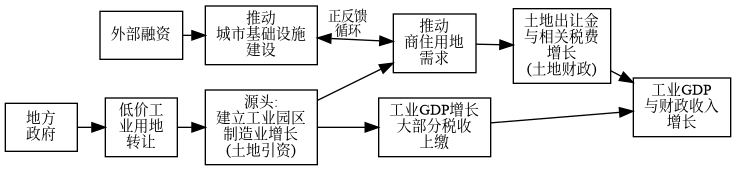
\includegraphics[width=0.9\textwidth]{figures/before08.png}
  \caption{\label{fig:bf08}2008年以前工业增长、土地财政与地区经济增长(可持
    续) }

  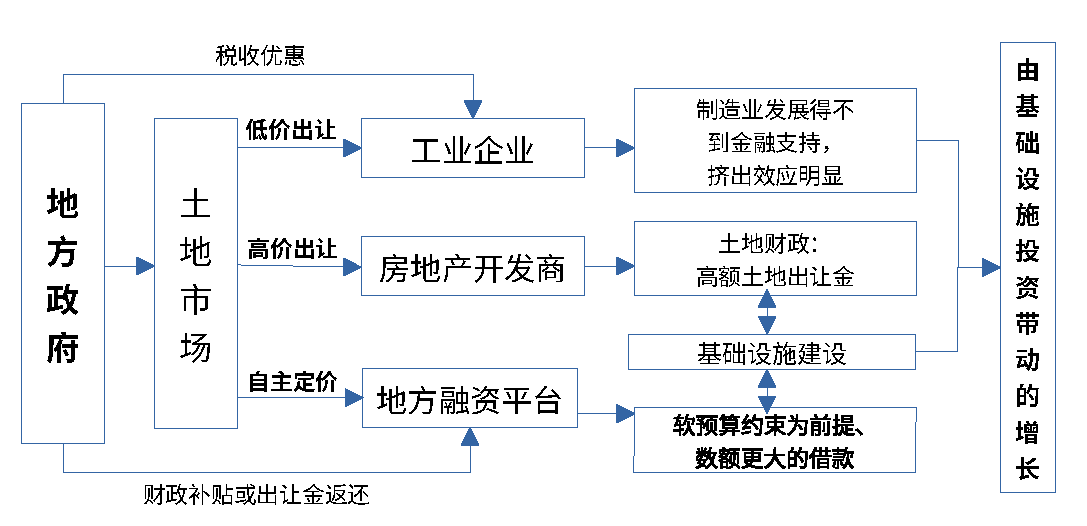
\includegraphics[width=0.9\textwidth]{figures/after08.pdf}
  \caption{\label{fig:af08}2008年后软预算约束与地区经济增长(不可持续) }
  \capsource{范剑勇\qquad《四万亿如何改变了中国经济增长动力》}
\end{figure}

据范剑勇\cite{fanjianyong}:
\begin{quotation}
  2008年之前,中国是硬预算约束条件的土地财政模式(见\cref{fig:bf08},而2008年
  之后,是软预算约束条件下的土地金融模式(见\cref{fig:af08}。2008年之前,经济
  增长的动力是“制造业+房地产”两个轮子一起转,2008年之后是偏向以基础设施为主
  的单轮驱动。
\end{quotation}

详细论述可见范原文,不再赘引。4万亿之后的土地金融历史,就本书所占角度来说,未发生
明显本质转变,也不再赘述。

\subsection{土地置换制度}

本小节几乎照摘周飞舟和谭飞智所著《当代中国的中央地方关系》。

自改革开放以来,我国工业化、城镇化推进速度越来越快,大量耕地农用地被占用是土
地财政\footnote{“土地财政”四字为笔者所加。}发展的必然要求。尤其是进入21世纪以来,
各地土地财政带来大拆大建,形成规模不小的失地农民群体,频发的群体性事件成为危
害社会稳定的重要因素。自中央层面来看,基于保障\textbf{国家粮食安全}以及维持改革以来
确立的家庭联产承包责任制的基本经营组织方式的要求,实行严格的耕地保护制度,以
占补平衡为代表的系列政策应运而生,\textbf{18亿亩耕地红线}作为一项政治任务贯穿而下,
实行一把手问责制。

\subsubsection{耕地占补平衡}

1997年4月,中共中央国务院发布11号文《关于进一步加强土地管理、切实保护耕地的通
知》,明确提出省(区市)必须保持耕地总量动态平衡的要求,同时确定了实行占用
耕地与开发复垦\footnote{土地复垦是指对生产建设活动和自然灾害损毁的土地,采取整治措施,
  使其达到可供利用状态的活动。}挂钩的政策,首次明确提出“耕地占补平衡”的概念。

随后在1998年8月,《中华人民共和国土地管理法》再次修订,明确提出“实行占用耕地
补偿制度”,要求占用耕地与开发复垦耕地相平衡。

1999年2月4日,《关于切实做好耕地占补平衡工作的通知》(国土资发〔1999〕39号)要
求确保建设占地“\textbf{占一补一}”,逐步实现耕地占用的\textbf{先补后占、占优补优、不补不
  占}。自此,耕地占补平衡政策开始在全国各地大规模实施。

2006年以前,占补平衡考核采取的是“\textbf{算大帐}”的方法——以区域为单位,考核区域内
的总占总补平衡。这种方法存在的漏洞是,很多建设用地项目并没有实现法律所规定的
占补平衡,建设用地占用耕地项目单位的补充耕地与土地开发整理脱钩。同时,由于区
域内的占补平衡考核仅仅关注于数量,一些建设项目\textbf{占优补劣}的现象比较突出。

2006年6月8日,国土资源部第3次部务会议通过了《耕地占补平衡考核办法》,于当
年8月1日起施行。“耕地占补平衡考核,\textbf{以建设用地项目为单位进行}”“耕地占补平
衡,实行占用耕地的\textbf{建设用地项目与补充耕地的土地开发整理项目挂钩}制度。”不再
采取大锅饭式的算大账。这一管理思路,为后来的增减挂钩所延续,即采用“\textbf{封闭运
  行}”的项目制运作模式,

随着工业化、城镇化的大势所趋,\textbf{“保耕地红线”成为地方政府沉重的政治负担和资金负
担。}耕地占补平衡政策自出台以来,在各地具体实施过程中主要存在:耕地的“\textbf{实占虚
补}”;补充耕地的“\textbf{实优虚劣}”以及\textbf{农地非农化和非粮化}的风险。耕地占补平衡制度实
行以来,各地实际工作中建设占用耕地长期以“先占后补”和“边占边补”方式为主,
加上对补充耕地的监督力度不够,导致建设占用耕地占而不补、占多补少的问题经常发
生。国土资源部因此颁布《关于进一步加强土地整理复垦开发工作的通知》,规定
从2009年开始,除国家重大工程可以暂缓外,非农占用耕地全面实行“\textbf{先补后占}”。

% 从地方政府角度出发,其更多的是从如何提高土地生产效益的角度出发的,因此如果单
% 纯地维持原有以粮食为主的种植结构难以达到提高效益的目的,转变生产结构成为必然
% 的选择,农地非农化、非粮化在所难免。所谓粮食安全的担忧也并非地方所考虑的问题。
% 在这一点上,中央与地方之间的矛盾凸显。

由于耕地的开垦整理需要一定的工程周期,因而由“先占后补”到“先补后占”的转变,
开启了\textbf{耕地占补平衡指标化}的进程,各地纷纷建立\textbf{占补平衡指标储备库}。提前储
备补充耕地,需新增建设用地时再从库中支取“指标”。

% 中国耕地红线粮食战略安全和土地金融的交织摩擦,使地区\textbf{狂热开发}建设用地的意
% 图受限\footnote{此句为笔者所加。以中国为一整体的角度来考虑,各地重复建设、大干快上,
% 工业用地扭曲的拿地或租赁价格、房地产的癫狂实属狂热无疑。},尤其是经济发达地
% 区与产粮大省更加受限于补充耕地资源较少。

% 从另一各方面来说,耕地红线也使可转化为新增建设用地的农地更加稀缺,加重了土地
% 金融的严重程度。\footnote{此句为笔者所加。}

\subsubsection{土地置换与指标折抵}

中央、省、市、县、乡五级政府的五级规划与年度建设占用耕地计划指标等限制了各级
地方政府对于新增建设用地、发展土地金融的强烈渴求,与中央严格土地制度框架出现
较尖锐矛盾,违法占地屡禁不止,中央政府为此开了以农用土地整理换取新增建设用地
的“口子”。

1999年10月,《国土资源部关于土地开发整理工作有关问题的通知》(国土资发
〔1999〕358号)提出土地置换和指标折抵。

\begin{description}
\item[土地置换] 促进农村居民点向中心村和集镇集中、乡镇企业向工业小区集中,选定新
  址\textbf{建设需要占用其他耕地}时,可以与腾出来的\textbf{旧址整理后增加的耕地}进行置换,实行
  这种方式置换的其建设用地\textbf{不占用年度建设占用耕地计划指标}。


\item[百分之六十指标折抵] 实现耕地占补平衡的地区,可以用通过土地整理\textbf{新增耕地面积
  的百分之六十指标},向上级土地行政主管部门申请一定数量的\textbf{预留建设占用耕地指标},
  用于本地区必需的非农建设。但必须按规划用地,并要严格检查,适当控制。
\end{description}

这两项政策“指标的使用并\textbf{不占用当年的年度建设用地指标},因而受到各地方政府的
欢迎……也是城乡建设用地增减挂钩政策出台的前奏”。

但地方政府仍感受到五级区域对于发展建设用地限制较大:发达地区可供补充耕地量匮
乏,不能满足新增建设用地需求;一般为10--15年的土地规划无法更好预见未来发展,
不可占用基本农田\footnote{基本农田:为了切实保护耕地,国家把按照一定时期人口和社会经
  济发展对农产品的需求,以及对建设用地的预测而确定的\textbf{长期或一定时期内不得占
    用的耕地}称为基本农田。}使大块建设用地项目难以落地。于是一些省开始省内跨
区域操作,实现了较为系统性变通的是浙江省,一些人称之为“\textbf{浙江模式}”。简而言
之就是浙江省将一些指标统筹在省或市以内,不下沉分解至各县各乡;并且各市之间可
以交易指标,落后地区大量土地整理用以补充耕地,发达地区向落后地区购买耕地指标
专心发展建设用地。详细了解可见汪晖、陶然《论土地发展权转移与交易的 “浙江模
式”——制度起源, 操作模式及其重要含义》。


\begin{quotation}
  对浙江在土地发展权转移和交易上的改革探索,不仅学界有论述质疑浙江的做法
  是\textbf{规避中央政府基本农田审批权和新增建设用地土地有偿使用费,导致基本农田质
    量下降和建设用地总量失控}(谭峻等,2004 年),中央政府也存在不少担心。

  欠发达地区为了折抵指标过度投资土地整理,甚至在新增耕地比例上弄虚作假,或发
  达地区通过购买折抵指标无限制扩张城市和工业园区用地。

  浙江省基本农田集中置换和易地代保政策\footnote{即基本农田易地代保:简而言之,发达市
    县有偿购买落后市县的基本农田,以便消除本市县相应面积、质量的基本农田保护,
    新增大块连续建设用地。}在国土资源部《关于进一步采取措施落实严格保护耕地制度的通
  知》(国土资发〔2003〕388 号和国务院办公厅《关于深入开展土地市场治理整顿严格
  土地管理的紧急通知》(国办发明电〔2004〕20 号)公布后停止执行;折抵指标政策也
  在《国务院办公厅关于严格执行有关农村集体建设用地法律和政策的通知》(国办发
  〔2007〕71 号)颁布后停止执行。\cite{wangzhejiang}
\end{quotation}


\todo[inline]{浙江模式其实就是市县级土地金融的扩大版,大国大城其实就是浙江模
  式的扩大版?参考LaTeX源文件中以下被注销部分。自由派认为行政主导要继续让位
  给市场自由流动。}

\subsubsection{城乡建设用地增减挂钩}

\begin{quotation}
  2004年10月21日国务院下发《关于深化改革严格土地管理的决定》,“实行最严格
  的土地管理制度……鼓励农村建设用地整理,\textbf{城镇建设用地}增加要与\textbf{农村建设用
    地}减少相挂钩”。

  (4年陆续增加试点后,)2008年6月27日,国土资源部印发《城乡建设用地增减挂钩
  试点管理办法》,明确提出了“城乡建设用地增减挂钩是指依据土地利用总体规
  划,\textbf{将若干拟整理复垦为耕地的农村建设用地地块(即拆旧地块)和拟用于城镇建
    设的地块(即建新地块)等面积共同组成建新拆旧项目区}(以下简称项目区),通
  过建新拆旧和土地整理复垦等措施,在保证项目区内各类土地面积平衡的基础上,最
  终实现\textbf{增加耕地有效面积,提高耕地质量,节约集约利用建设用地,城乡用地布局更
  合理}的目标。”其实仔细比较增减挂钩政策与之前我们所分析的建设用地指标置换政
  策其在表述上和本质上相类似,而这也反映了中国改革中政策制定的延续性和探索性。

  同时138号文批复下达了第二批试点项目(共10246公顷,合15.368万亩),项目区以
  项目区备选方式下达。2009年3月5日,《国土资源部关于2009年第一批城乡建设用地
  增减相挂钩周转指标的批复》(国土资函[2009]299号),对河北、内蒙古、辽宁、吉
  林、黑龙江、福建、江西、河南、湖南、广东、广西、云南、宁夏13省(区),批复
  下达周转指标15.275万亩(合10183.3公顷)。2013年10月23日下午,国土资源部部长、
  党组书记、国家土地总督察姜大明主持召开第15次部长办公会,审议并原则通
  过2013年城乡建设用地增减挂钩指标分解下达方案,共批准29个省份开展增减挂钩试
  点,全国共安排城乡建设用地增减挂钩指标90万亩。\cite{yangdi}
\end{quotation}

\begin{figure}[htbp!]
  \centering
  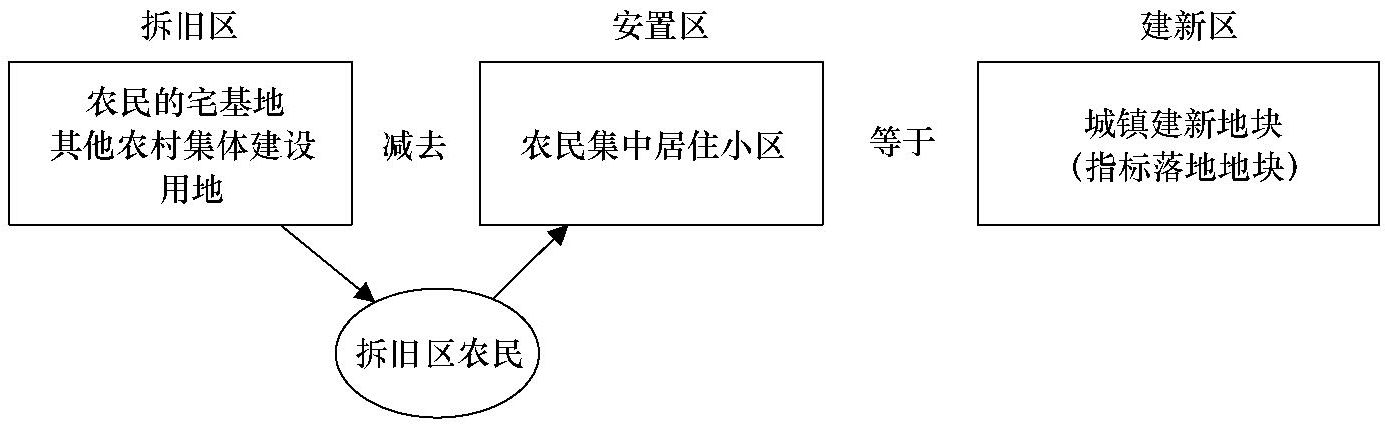
\includegraphics[width=0.9\linewidth]{figures/zengjianguagou.jpg}
  \caption{\label{fig:zengjianguagou}城乡建设用地增减挂钩政策示意图}
  \capsource{周飞舟、谭飞智\quad 《当代中国的中央地方关系》}
\end{figure}

\begin{quotation}
  指标计算公式:增减挂钩周转指标=拆旧区总面积-农民集中居住小区占地面积=项目区
  中建新地块可占地面积(见\cref{fig:zengjianguagou})。所谓“\textbf{周转指标}”其
  在实质上是一种指标“\textbf{预借}”或“\textbf{透支}”制度。拆旧复垦是一项非常庞大的工
  程,短期内难以完成,因此不需要拆旧区完成耕地复垦工作之后,建新区才能够进行
  城镇开发建设。也正是在这个意义上才有了指标“\textbf{周转}”的概念,一般要求,指标
  三年归还。

  增减挂钩的根本意义在于:开辟了一个独立于每年新增建设用地指标严控体系以外的
  指标来源,为城镇发展提供“不占指标”的“计划外”土地资源,且规模逐年增加。\cite{yangdi}


  截至2013年底,全国共有29个省(自治区、直辖市)被纳入了试点范围,共下达周转
  指标约90万亩。

  2017年4月,增减挂钩再出新政,在《关于进一步运用增减挂钩政策支持脱贫攻坚的通知》
  中,明确允许省级贫困县的增减挂钩节余指标在\textbf{省域范围内}流转使用,进一步释放了
  政策红利。为了落实国家乡村振兴战略,2018年3月,国务院办公厅印发了《城乡建设用
  地增减挂钩节余指标跨省域调剂管理办法》,规范了“三区三州”及其他深度贫困县增
  减挂钩节余指标\textbf{跨省域调剂},助力落实国家精准扶贫、绿色发展的战略。至此,增减
  挂钩先后两次完成政策升级,从省域内流转到跨省调剂,逐步拓展政策适用范围。这一
  阶段增减挂钩政策更加强调以人为本,致力于城乡区域协调发展和社会公
  平。\cite{zengjianzongshu}
\end{quotation}

据《央地关系》,不管是政策实质还是地方需求,对新增耕地并无多少刺激,只是满
足“占补平衡”即可。如\cref{fig:zengjianguagou},为获得更多新增建设用地,地方
倾向于减少农民集中居住小区占地面积,显而易见的方法是“农民上楼”——楼房可以
在单位占地面积提供更大容积率、容纳更多被增减挂钩析出的农民;并采用合村并居等
方法,以便进一步减少成本、扩大新增建设用地指标。

中央中央政府面临对地方监管失控的风险。一方面土地金融下,地方为GDP考核机制不满
足于中央给定的增减挂钩指标,为获得更多新增建设用地或直接将用地指标出售给其他地
方,对大量村庄违规改造;另一方面中央为维持地方发展的积极性及活力,又不得不逐
年扩大试点范围和规模。

增减挂钩以项目制方式向下推进,中央资金以项目形式向下转移,各级地方政府必须要
有相应的配套资金和政策支持,地方政府继续高额举债以及引入社会资本成为必然。债
务压力迫使地方忽视了反哺农业、农村、农民,仍倾向于以建设养建设;可同时进行的
拆旧和建新在极端情况下也会停滞或缓慢发展,造成各种不安定因素积累发酵;地方也
面临和社会资本的博弈;合村也带来更多政治管理矛盾。

起初农村拆迁矛盾多因行政强制指令下补偿不足,农地价征收城低价出售,城乡二元对
立有所加重,有损村民利益。随着政府日益重视农民权益问题,拆迁补偿已有较大实质
性改观。但随着市场经济边沁利己的日益深入人心,土地金融的日益发展,使土地成为
全民全社会共同参与的虚假繁荣市场,增减挂钩成本日益提高,越发加重了风险。


土地金融造成地方各自为政,产业结构相同且全副该,重复建设,狂热追求新增建设用地,农民上楼,大额投资等等


韩长赋: 中国农村土地制度改革

耕地退化、污染严重,一些地方占好地、补坏地,占水地、补旱地,2016 年全国优高
等耕地面积仅占 29. 5%。




反面论述
https://www.aisixiang.com/data/115819.html
赵燕菁:从土地金融到土地财政:资本的胜利、有为的政府与城市的转型

※※※※※※※※※※※※※※※※※※※※※※※※※※
https://bfi.uchicago.edu/wp-content/uploads/2022/02/BFI_WP_2022-24.pdf

文献中的典型观点是,住宅用地出让主要是地方政府增加收入的一种方式,而工业用地
出卖主要是为了补贴产业、刺激经济增长、支持劳动力需求。

中国的土地市场具有相当大的工业折扣:工业区用地比住宅用地便宜一个数量级。与以
产业补贴或促进产业增长为中心的解释相反,我们强调了未来土地税收的重要性,并发
现地方公共财政激励措施可以在很大程度上合理化这种价格差距。在“土地融资”制度
下,土地出让是中国地方政府的重要收入来源。研究表明,在中国,地方政府作为垄断
性土地销售者,面临着住宅用地或工业用地供应之间的权衡,这取决于工业和住宅用地
销售收入的不同时间分布、地方政府的财政约束以及地方政府与其他各级政府分享税收
的程度。

公司税收收入和土地出让收入;2019年,这两个数字分别约为8.7万亿元人民币和7.3万
亿元人民币.2工业用地产生持续的未来税收流动,因为工业企业缴纳增值税和所得税,
以及各种费用。由于中国没有住宅物业税,住宅用地销售只会暂时增加房屋开发商缴纳
的税款.3这意味着地方政府面临着一个选择,即出售前期收入较大的住宅用地和出售工
业用地,因为工业用地支付的税收现金流比实际收入更持久。

这种动态的观点意味着,大量的前期工业用地折扣并不一定意味着政府正在通过廉价土
地系统地补贴工业。事实上,我们表明,在调整住宅开发商缴纳的税款后,来自工业用
地的税收流动可以定量补偿前期工业用地折扣。我们还提供了地方政府的融资需求影响
土地分区的因果证据,表明地方公共财政在通过土地分配渠道塑造中国经济增长路径方
面发挥着被低估的作用

我们从一个概念框架开始,分析推动工业用地而不是住宅用地供应均衡回报的力量。我
们考虑的是地方政府,其目标是最大化其财政收入的现值。除了全部属于地方政府的前
期土地销售收入外,住宅用地还产生了由房屋开发商支付的一次性税款,而工业用地则
产生了工业税的持续现金流,并与中央政府共享。在均衡状态下,由于未来的税收优惠,
当地政府愿意以较低的价格出售工业用地。该框架指出了两个简单且可衡量的汇总统计
数据。首先是工业折扣,即工业用地和住宅用地之间的价格差异。第二种是工业用地销
售的内部收益率(IRR),计算为贴现率,折现率等于工业和住宅用地销售的所有现金
流的现值

※※※※※※※※※※※※※※※※※※※※※※※※※※

就像许多其他国家一样,中国也有严格的分区限制。正如Chen等人(2018)所强调的那
样,划为住宅用途的土地的售价大约比划为工业用途的土地高出十倍。2019年,中国住
宅用地平均价格为3,619元/平方米,工业用地平均价格为304元/平方米。我们将住宅用
地和工业用地之间的这种价格差异称为工业用地折扣(或工业用地互换)。

※※※※※※※※※※※※※※※※※※※※※※※※※※

地方政府从土地中获取融资有两条直接渠道:一是土地财政,即通过出让国有土地(主
要是商服用地和住宅用地)50至70年的使用权来获取级差地租;二是土地金融,即将土
地注入地方融资平台来撬动资金为城市建设融资。

已有研究表明,土地财政和土地金融相结合的以地融资模式催生出一个高效的融资体系,
极大推动了近二十年来的中国经济增长,特别是与房地产和基建相关(包括钢铁、水泥)
的重工业部门得到了飞速发展,居住环境和基础设施的改善又进一步促进了地价和房价
的升值,为下一轮以地融资创造了有利条件。这样的正向反馈机制使得中国自1998年以
来一直处于投资驱动型的增长阶段。

如果说曾经的以地融资模式主要依赖土地财政,那么如今,随着部分地区土地资源的告
罄和征地补偿标准的提升,一些地方政府对土地财政的依赖开始减退,而对土地金融却
愈加青睐。由表1可知,越是土地资源稀缺的地区(东部地区),土地抵押贷款规模越
是高于土地出让规模,而对北上广这样的一线城市而言,土地抵押与土地出让的比值更
是高于东部地区的平均水平。

图1显示,2003至2010年间,出让成本占比基本维持在六成左右,但在2011至2018年间,无论是土地出让成本的规模还是其占土地出让毛收入的比重都呈加速上升趋势,甚至到了2018年,土地出让成本占土地出让毛收入比重已接近九成。

从征地规模的角度亦可佐证土地出让成本在2010年前后出现了飘升的现象。图2显示,农用地和总的土地征收规模在2011年之前处于上升区间,但在2011年后呈逐年加速下滑的态势,这恰好是土地出让成本开始飘升的年份(参见图1)。迅速缩小的征地规模表明,未来国有土地的出让规模将大幅缩减,利用土地财政进行创收的空间将被进一步压缩。

1994年的税收分享改革,该改革减少了地方政府在许多税收收入来源中的份额,同时并没有减少他们的支出需求。要回答“为什么土地金融在中国(到目前为止)有效运作”要复杂得多。在这方面,了解其促进土地金融体系盈利能力的制度基础是很重要的。首先,地方政府被指定为地方城市LUR的垄断提供者。因此,当一个城市提出购买农村土地并将其转换为城市土地时,它不会面临来自其他实体的竞争。此外,支付的补偿是基于当前(农业)用途的土地价值,而不是未来城市用途。地方政府回购、分配或出售的城市土地利用率并将其转换为新的土地利用率时,也适用类似的规定。这种安排使城市政府能够获利,直到最近,土地价格的暂时上升趋势加剧了这一点。值得注意的是,支撑土地金融体系的丰富制度框架既有法律、官方文件等显性规则,也有在实践中具有影响力的隐性规范。其中一些细节在现有文献中似乎没有得到适当的承认,并可能导致对该系统的误解。希望我们的分析能够更清楚地说明该系统在中国联邦体系中的运作方式

自1980年代以来,中央和地方政府在中国经济中扮演的角色已经很明确——中央政府负责规划和监管,而地方政府则负责在地方层面实施这些法规。

从1980年到2020年,地方政府在国家一般公共预算中的份额从45.7\%增加到85.7\%,而同期收入在一般公共预算中的份额从75.5\%下降到55.5\%。为了弥补收支缺口,地方政府依靠中央政府补贴、债务融资和土地融资。

1994年实行的税制改革在随后的几年中对土地融资产生了巨大的溢出效应。改革规定,中央政府将把所有与土地有关的税收分配给地方政府。这包括土地价值税、城市土地使用税、耕地占用税、土地增值税、契税(财产转让税)和一般财产税。更重要的是,土地出让的所有利润都转移到了地方政府。

这一新制度为地方政府增加了土地出让收入提供了强大的动力。从2000年到2020年,地方政府土地出让收入占总收入的比重从5.9\%提高到42\%。如果将其他相关的土地税也考虑在内,土地收入占地方政府总收入的一半以上(52\%)。

o“通过信用制度,未来的收益可以贴现到今天,使得资本的形成方式得以摆脱对过去积累依赖,转向预期收益。”“中国城市伟大成就背后的真正秘密,就是创造性地发展出一套将土地作为信用基础的制度——‘土地财政’。”


土地财政是指政府出让国有土地使用权收入,及与土地有关的税收如耕地占用税、土地增值税等,这都是有法律、制度依据的。土地金融是指政府拿土地做抵押,向银行贷款,属于政府负债。这样做,没有法律依据,是打了制度的“擦边球”,因为制度允许政府作为国有土地所有权的代表经营土地。


但是当市场经济更多要求个人为个人负责,并将此观念植入人心时,一些原住民的死缠
烂打、坐地起价也就避无可避,因此拆迁往往要大费周章。突破口似乎只有合法或非法
的“暴力”。

合法暴力,可以宣称土地权利不归属于抗拒拆迁的人员,如印度最高法院声称孟买等地
贫民窟的长期居民是土地的非法占有者,没有权利要求拆迁赔偿,\textbf{承认获赔权等于奖
励盗窃行为};美国滥用征地权,把合理建筑中的长期居民赶走,鼓励高层建筑;声称
土地为集体所有,集体才是土地权利所有者,而非小部分人。

非法暴力,如20世纪90年代韩国首尔开发商雇佣黑帮“相扑似的打手”暴力拆迁;印度
西孟加拉邦南迪格莱姆地区的冲突惨案等。


《从沸腾到癫狂》

北京2005~2009年政府公布的商品房住宅建设用地计划供给指标为7130公顷,非商品住
房建设用地指标为1320公顷,两者的比重为5.4∶1。而实际供给的情况则是,商品房住
宅用地(招拍挂)2394公顷,完成计划数的33.6%,供地差额为4736公顷;非商品住宅
供地1283公顷,完成97.20%,扣除商品房中的配建,非商品房完成率为103%。这些土
地为享受经济适用住房政策的用地,约为商品房用地的2倍,由特定单位使用了。商品住
宅用地与非商品住宅用地的面积相加,可以计算出商品住宅用地在全部住宅建设用地中
的比重仅为28.3%。



任志强认为,市场中计算出的商品住宅平均销售价格仅为这28.3%的住宅销售价格,而并非北京市的住宅实际价格。如果用地中的平均容积率相等,且大部分经济适用住房和享受经济适用住房政策的住房价格为4500元/平方米,则北京市的一手房销售价格约仅为6200元/平方米。

任志强说,虽然那些低价的定向住房没有向社会公开销售,比如分给了国务院事务管理局,再分配给中央或国务院的各机关、管理机构以解决公务员的住房、进京干部的住房、老干部的住房等,但这些住房也是解决北京的住房问题,所以,应该在统计时计算进来进行平均。

房真实房价平均仅为6200元/平方米。而根据北京市统计局、国家统计局北京调查总队公布的《2009年北京市房地产市场运行情况》,2009年第四季度,四环路以内商品住宅期房销售均价为25907元/平方米。

6200元/平方米与25907元/平方米,为什么两者的差距如此之大?



任志强如是写道:



北京2005~2009年政府公布的商品房住宅建设用地计划供给指标为7130公顷,非商品住房建设用地指标为1320公顷,两者的比重为5.4∶1。而实际供给的情况则是,商品房住宅用地(招拍挂)2394公顷,完成计划数的33.6%,供地差额为4736公顷;非商品住宅供地1283公顷,完成97.20%,扣除商品房中的配建,非商品房完成率为103%。这些土地为享受经济适用住房政策的用地,约为商品房用地的2倍,由特定单位使用了。商品住宅用地与非商品住宅用地的面积相加,可以计算出商品住宅用地在全部住宅建设用地中的比重仅为28.3%。



任志强认为,市场中计算出的商品住宅平均销售价格仅为这28.3%的住宅销售价格,而并非北京市的住宅实际价格。如果用地中的平均容积率相等,且大部分经济适用住房和享受经济适用住房政策的住房价格为4500元/平方米,则北京市的一手房销售价格约仅为6200元/平方米。

任志强说,虽然那些低价的定向住房没有向社会公开销售,比如分给了国务院事务管理局,再分配给中央或国务院的各机关、管理机构以解决公务员的住房、进京干部的住房、老干部的住房等,但这些住房也是解决北京的住房问题,所以,应该在统计时计算进来进行平均。

按照任志强的说法,商品住宅用地28.3%之外的用地,一部分被用于建设北京市和在京中央和国家机关的公务员住房,他们的名称可以是两限房、经济适用住房、享受经济适用住房政策的住房、合建房、自建房中的任何一个。当然,也不排除这些公务员在享受了经济适用房等保障房以后,仍然自掏腰包去购买商品房。



地产商什么时候成为一个阶层了?正统的社会学者肯定要嘲笑我的无知。他们会教育我:你可以称他们为一个群体,一个集团,就是不能称其为一个阶层。是啊,连天天挂在老百姓嘴边的“中产阶层”都未获正式承认,哪里来的地产商阶层?

为什么地方政府会产生对土地财政像网瘾一样的依赖?根子在于土地招拍挂制度。这是一个影响力仅次于1998年房改的制度,并将继续对房地产市场和地方财政产生决定性的导向作用。

招拍挂制度必然导致地价上涨,而地价上涨则必然推动房价上涨。只要招拍挂制度存在,地王的产生就不可避免。地产GDP主义是被一种强力制度牢牢地固定住的地方政府价值取向。

并于2010年6月后成功超过日本成为全球第二大经济体,其中房地产贡献良多。据国家统计局数据,2010年,全国房地产开发投资完成48267亿元,同比增长33.2%;全国商品房销售面积10.43亿平方米,同比增长10.1%;商品房销售额约为5.25万亿元,同比增长18.3%。

因此,即使是全面调控的2010年,房地产的地位也丝毫没有下降。自从1998年实行住房商品化以后,GDP对房地产业的依赖就逐步形成,以至于到了离不开的地步,关键时刻总是要靠房地产“挺身救主”。实事求是地说,这方面没有一个产业能比得上房地产。

以上是从全局,从中央政府层面来说。对地方政府来说,房地产就更重要了。土地财政,这已成为大多数地方政府最重要的财政收入来源。城市形象、政绩工程也离不开地产商和房地产业,许多地方的道路等基础设施都是由地产商修建的。

2004年以来,地方政府体会到土地公开出让的无可替代的好处,招拍挂出让普遍推行。而招拍挂一般是净地出让,拆迁是政府的事。而土地收益当然要远大于拆迁补偿款,否则他们是没动力拆的。地方政府为了尽快把土地卖出去,就会做出强制拆迁、暴力拆迁的事情来。


1991年实施和2001年修改的《城市房屋拆迁管理条例》。依此条例,地方政府贴一纸拆迁通知,在被拆迁的房屋上圈画一个大大的“拆”字就够了。居民不肯搬迁?先有房管部门行政裁决强制拆迁;还不服?接着可能就是法院裁决直接带着铲车来。许多地方连行政和法院裁决都懒得走,直接派消防队和铲车来。这才叫雷厉风行,超级效率。中国城市面貌的日新月异,城市建设的突飞猛进,该《条例》立了大功。

不少专家称这部条例是一部恶法,出台伊始就呼吁修改之。修改后的条例草案数易其稿,并分别于2010年1月29日和12月15日分两次向全社会公开征求意见,这在我国立法史上前所未有,也从一个侧面证明了拆迁所涉及的利益极为纷繁复杂。北大法学教授说,新的条例难以正式出台,主要就是遭遇到地方政府的强烈阻挠。千呼万唤之后,2011年1月21日,国务院正式出台《国有土地上房屋征收与补偿条例》。



2007年1月,国家税务总局曾要求各地税务机关严格土地增值税清算,此举曾令开发商大
为紧张。然而,金融危机呼啸而来,经济形势急转直下,这一号称“革房地产商命”的
税收政策再一次不了了之。赵晓等吁请严征土地增值税,以“100%预征、100%清
算”来遏制新一轮楼市疯狂。

到遏制投机的作用一样,对地产商和投资者个人尤其是地产商征收土地增值税,亦未能成为阻止涨价的动力。

事实上,土地增值税更像是为地方政府找到了一个新的税收来源,虽然这可能并非该税种设立的初衷。

严格征收土地增值税,能够为地方政府带来多大的税收?实事求是地说,2010年以来的保障房建设规模,令人惊讶。

很难想象,如果没有2008年10月推出的4万亿政府投资计划,保障房建设会有今天如此庞大的规模。我并不是说加快保障房建设是为了应对国际金融危机而采取的措施,而是说,保障房建设规模如此庞大,沾了4万亿“救市”资金的光。

2008年11月5日召开的国务院常务会议,确定了进一步扩大内需、促进经济增长的十项措施(“出手要快,出拳要重”的说法由此而来),第一条就是加快建设保障性安居工程。在4万亿投资里,坊间曾有保障房占8000亿元、9000亿元的说法,但并不准确。

根据国家发改委主任张平2009年3月8日在十一届全国人大二次会议新闻发布会的介绍,在4万亿政府投资计划中,保障性住房投资总规模为4000亿元左右。从张平的介绍来看,保障房包括廉租房、林区、垦区、煤矿棚户区改造,但没有提到限价房、经济适用房、公共租赁房等的投资,所以实际投资规模要远远大于4000亿元。

2008年受国际金融危机影响,除北京等极个别城市外,各地对保障房投入仍然不足。真正较大规模的保障房建设是从2009年开始的。

根据2010年3月5日全国“两会”上的《政府工作报告》,2009年中央财政安排保障性安居工程补助资金551亿元,比上年增长2倍。新建、改扩建各类保障性住房200万套,棚户区改造解决住房130万套。从中央财政投入看,增幅甚大。那么,2009年地方对保障房的投入有多少呢?

全国人大常委会专题调研组2009年10月月底披露的一份调查报告显示,截至当年8月月底,全国保障性住房建设完成投资394.9亿元,完成率仅为23.6%。以此推算,当年全国保障房投资计划大约为1600亿元。减去中央财政投入的551亿元,地方即使足额完成投入计划,亦不过1050亿元。

财政部2007年11月颁布的《廉租住房保障资金管理办法》规定,应从土地出让净收益中按照不低于10%的比例安排用于廉租住房保障资金。2009年全国土地收益实际到账14239亿元。也就是说,2009年各地仅廉租房就应投入1424亿元。加上公共租赁房、经济适用房和限价房,总投入至少应该倍增。而事实上,2009年各地保障房实际投入额尚不足财政部规定的廉租房投入额,遑论加上公共租赁房、经济适用房和限价房。

当然,从全国“两会”《政府工作报告》公布的数据看,2009年全国保障房建设任务是完成了的。330万套保障房的投资,应远远超过1600亿元。

2010年的保障房建设规模更加惊人。根据住房和城乡建设部的安排,2010年全国计划建设廉租住房、公共租赁住房等300万套,改造各类棚户区住房280万套,农村危房改造试点120万户。农村危房改造不计,人们将2010年的保障房任务简称为580万套。从330万套,到580万套,增长超过70%。

https://www.mof.gov.cn/zhuantihuigu/czjbqk2011/czsr2011/201208/t20120831_679821.html
全国土地出让收入管理及使用情况

2007年之前,土地出让收入先纳入预算外专户管理,再将扣除征地补偿和拆迁费用以及
土地开发支出等成本性支出后的余额缴入地方国库,纳入地方政府性基金预算管理。
从2007年开始,国家对土地出让收入管理制度进行了改革,将全部土地出让收入缴入地
方国库,纳入地方政府性基金预算管理,与公共财政预算分开核算,专款专用。土地出
让收支纳入政府性基金预决算编制范围,实行预决算管理制度。每年第三季度,国土资
源管理等有关部门按照相关规定编制下一年度土地出让收支预算。每年年度终了,国土
资源管理等有关部门按照规定编制上年土地出让收支决算。同时,按照规定程序向同级
人民政府报告,政府依法向同级人大报告。

% 新自由主义,彻底的附庸
% 杨继绳《中国改革时代的政治斗争》
% \begin{quotation}

% 新左派认为,目前中国的改革越来越走向自由主义所倡导的模式,中国正在进入资本主义全球体系。当前“中国社会的各种行为,包括经济、政治和文化行为甚至政府行为,都深刻地受制于资本和市场活动。”“80年代中国的启蒙思想所许诺的‘好社会’不仅没有伴随经济市场化而到来,市场社会本身呈现了新的、在某种意义上来说是更加难以克服的矛盾。”(汪晖:《当代中国思想状况和现代性问题》)新左派满怀忧虑地问道:“我们今天这个世界究竟是谁在统治,是人民呢还是寡头?是权力呢还是资本?这是需要深思的。在全球化潮流下,跨国公司正在系统地、有步骤地剥夺世界各国人民的民主权利,正在把我们这个世界带向奴役之路。如果看不到这一现实的威胁,恐怕就谈不上懂得民主。“(韩德强,2000)

% 自由派认为,目前中国虽然存在种种问题,但正在从不合理的体制走向合理的体制,走向人类文明的主流。他们所说的人类文明的主流就是以英美为标志的价值体系和社会制度。“对于自由主义立场而言,中国向市场经济转型问题再多再严重,也只能硬着头皮向前走,决不能走回头路,决不能返回衣、食、往、行都被人包办,种什么,造什么,卖什么都得等上级指示的那种日子。”(徐友渔:《自由主义与当代中国》)

% 对当前的社会结构的变化,自由主义者持乐观的态度。他们认为,20年的改革,已经在政府之外开始出现了新的社会结构,这种新的社会结构可能是将来中国的市民社会和公共领域的雏形,在中国的社会发展中是将成为一支重要力量。因此,让这种新的社会结构进一步发展是一条必由之路。新左派认为上述看法是当今既得利益集团虚构的神话,他们认为,这20年所形成的不是中间阶层,而是新生的资产阶,是垄断精英,垄断精英是改革中社会不公正的既得利益者,是需要限制的、而不是应当鼓励发展的阶层。

% 中国正处在十字路口,搞得好,就可能建成一个民主、法治的社会,搞不好,就可能形成一个金权、家庭统治的新型专制制度。就像某些南亚和拉美国家一样。这是两派一致的看法。但是,新左派认为这种危险在于市场霸权和垄断精英,自由主义者认为这种危险在于没有得到改革的原有的权力结构,在于中国两千多年相沿成习的专制主义。

% 自由主义者把政治权力的无限膨胀看成是奴役民众的力量,新左派把市场力量的无限膨胀看成是奴役民众的力量。
% \end{quotation}


% #+BEGIN_SRC dot :file before08.png :cmdline -Kdot -Tpng :exports results
%   digraph G {
%     rankdir="LR"
%     rank=min
%     ranksep=0
%     node[shape=record fontsize=11]
%     yuan[label="源头:\n建立工业园区\n制造业增长\n(土地引资)"]
%     shangzhu[label="推动\n商住用地\n需求"]
%     jishe[label="推动\n城市基础设施\n建设"]
%     end[label="工业GDP\n与财政收入\n增长"]
%     gongshui[label="工业GDP增长\n大部分税收\n上缴"]

%    外部融资 ->  jishe
%    jishe -> shangzhu[dir=both, label="正反馈\n循环", fontsize=10]
%    shangzhu -> "土地出让金\n与相关税费\n增长\n(土地财政)" -> end

%     "地方\n政府" -> "低价工\n业用地\n转让" -> yuan -> gongshui ->end

%     yuan -> shangzhu
%     {rank=same gongshui  shangzhu}
%   }
% #+END_SRC

%%% Local Variables:
%%% mode: latex
%%% TeX-master: "../main"
%%% End:




% 朱镕基是坦诚的,地方政府财政在民生上的捉襟见肘和土地财政问题 并不是完全由分税制造成的。李郇、洪国志、黄亮雄考察1999-2008年间,240个地级市地方财政预算内缺口和土地财政的关系发现,地方财政预算内缺口并不能完全解释土地财政的关系。

% 只有1999-2003年间,随着地方预算内缺口扩大,土地财政的规模才开始在不断扩大;
% 而2003年之后,地方预算内的切口是比较稳定的,但是土地财政的规模却在飞速膨胀。
% 这就说明20003年后,财政压力并不能解释地方对于土地财政的疯狂。

% 2003年是极为关键的一年,土地财政的起飞更多是因为2002年有两项政策,《招标拍卖挂牌
% 出让国有土地使用权的规定》和 企业和个人所得税改革。前者开了口子,地方政府可以通过
% 土地挂牌拍卖,从市场拿钱;后者就给了地方政府一鞭子,中央和地方以60\%:40\%的比例
% 来分企业和个人所得税增量。

% 2001年,地方所得税是1636亿,占地方总收入的21\%。被中央拿掉大头之后,地方自然对营业税的依赖进一步上升。 而建筑业又是营业税的第一大户,自此之后,地方政府盯着上房地产,疯狂的发展房地产也就不奇怪了。


% 2003年,个人所得税改革和土地挂牌拍卖合法化,潘多拉的魔盒正式被打开,土地财政和各个地方政府领导的晋升冲动产生化学反应,固定资产投资飙升,房地产开始起飞,中国经济逐渐开始出现过热的情况。 2003-2006年,每年的 GDP 增长都在10\%以上,中央又开始和地方展开新一轮的博弈,宏观调控,为过热的经济降温。

% 2010年前后,东部开始讲产业升级,腾笼换鸟,中西部就开始蠢蠢欲动。

% 2007年,郑州就已经成立专门针对富士康的招商工作领导小组,市长亲自任组长。可惜,富士康仍在鼎盛,省级领导时常来亲自拜访,市级领导还常常被拦在门外,郑州并没有任何特殊的待遇,只能时断时续的联系着。2010年,富士康跳楼事件发酵,传出北迁的消息,郑州又兴奋了起来,不过它只是其中的一个,当时还有廊坊、武汉、成都、烟台等许多内陆城市翘首以盼。

% 最后,郑州给出了极为优厚的条件,五免五减半;降低每年的社保和其他费用1亿美元,享受出口退税。5年之后,当传出中央开始清理税收优惠的消息,郭台铭这回就积极主动地多,还亲自去郑州拜会市长马懿,确认有关50亿的财政补贴的落实。


% 2012年,三星传出要考虑在海外投资300亿美元建厂, 西安就曾靠着天量的补贴,在北京和重庆的手中,抢下了三星300亿美金的高端储存芯片项目。

% 在最后2012年4月2日,三星确定项目落户西安的时候,一片哗然,众人纷纷猜测地方政府的补贴力度到底有多强。

% 媒体一度流传出,2000亿数字的嫁妆:投资30\%的补贴,“十免十减半”,修建配套措施,无偿提供土地。 众人惊呼,赔本做买卖。娄勤俭亲自上了凤凰卫视的《神州问答》节目解释,不做亏本买卖,没有“十免十减半”的政策,只是有“五免五减半”,而且是国家的政策,西安只承担运输成本费用。娄省长最后话里还是留了余地,即使不赚钱,

% “但是将有260多家配套企业过来,现在就已经有近100多家企业,跟着来投资,这就是一种增值效应,产业带起来了”。

% 2012年,中央以减税的名义提出营业税改增值税的政策,理由是消除第三产业重复征税,总理亲自赴沪督军。
% 中央如此劳心费神,自然也别有深意。中国经济的顽疾,是地方政府对于房地产、建筑业的依赖。房地产和建筑业除了能快速拉高 GDP 之外,还是营业税的主要来源,而营业税又是地方政府的主要税种,所以造成了地方政府受到税收激励偏爱房地产。

% 2016年5月1日,房地产、建筑业等营业税的主体税种纳入营改增,中央和地方的博弈达到高潮。 2016年3-4月,总理在一个月之内,连开了三次会来讲营改增的重要性。

% 中央拿了营改增拿掉营业税,自然对地方也要所交代,这也就是给地方开的房地产税。房地产税并不是房产税,房产税是一个已经存在的税种,只是一直免征罢了,而房产地产税是指整合房产税和城市土地使用税的新税种。

% 2017年4月7日,教育部就出台多校划片的政策以朝阳区为试点,规定6月30日之后拿到房产证的,参加多校划区的曾策,希望能够通过增加购买学区房的不确定性来降低房价, 可是刚刚买房的家长,就去教育部门抗议,指责教育部违反义务教育法中,“免试就近入学、学区制和九年一贯对口招生”的规定, 后来多校划片的政策也就不了了之了。

% 财权与事权相匹配”是分税制的基本原则,有多少钱办多少事。但这种政策有着严格的限制条件,即辖区内经济发展水平的同质化。在中国这样一个大国,各地的经济发展条件和能力并不均衡。2007年,党的十七大报告采纳了“财力与事权相匹配”的提议。

% 另一句叫做“上面千根线,基层一根针”——上面出政策,下面对口执行,任务最终都压到基层政府,形成“财权层层上收,事权层层下移”的局面。比如“中央点菜,基层埋单”,中央部委下发文件要搞新农合医保、农村危房改造等,地方政府就要掏钱。

% “最弱小的一级政府却承担着具有全局意义的支付责任。”天津财经大学教授李炜光评论说。这种体制使县乡两级政府承担了地方的多项公共服务责任。全国两千多个县级组织,曾经有一半以上拖欠教师和离退休人员工资,或大面积拖欠银行贷款和建筑工程款,以至于中央财政亲自出手,出台“三奖一补”政策(指中央对地方缓解县乡财政困难奖励和补助的办法)为此兜底。

% “从决策权来看,中国是全世界最集权的国家,从执行权来看,我们又是最分权的国家。”刘尚希说。

% 在刘尚希看来,造成这一现象的根本原因是,“地方政府只对本级财政负责,它对下没有责任,不愿下移财力,还‘市刮县’向下摊派等”。因此,他开出的改革药方是摈弃“层级财政责任制”,建立“辖区责任制”,即上级政府要对辖区内各级政府的横向和纵向财政平衡负责。比如县一级财政发不出工资,首先应该问责市政府或省政府,而不是由中央财政埋单。



% \begin{figure}[!p]
  \centering

  \begin{tikzpicture}[baseline]
    \begin{axis}[width=15cm,height=6cm,% no markers,
      every axis/.append style={line width=.8pt},
      cycle list={
        {blue,mark=*},
        {red,mark=square},
        {orange,mark=o},
        % {loosely dotted,mark=+},
        {green!90!black,mark=otimes*,
          mark options={fill=brown!40},
        }% <-- don’t add a comma here
      },
      xtick=data,
      % xticklabels={1975,1980,...,2020},
      xmin=1979,
      xmax=2018,
      xticklabel style= {/pgf/number format/1000 sep=,xshift=1ex, rotate=60,anchor=east,},
      ytick distance=0.5,
      % ytick=data,
      % yticklabels={0.1, 0.2, 0.3, 0.4, 0.5, 0.6},
      % extra y ticks={0.1,0.2,0.3,0.6},
      % extra y tick style={grid=major},
      % extra y tick labels={0.1, 0.2, 0.3, 0.6},
      xlabel=年份,
      ylabel=产量(亿吨),
      % grid=major,
      ymajorgrids,
      ]
      % \addplot+ [point meta=explicit symbolic, every node near coord/.append style={color=red}, nodes near coords,]
      \addplot table [x=totalyear, y=total, col sep=comma] {figures/econohistory/realliangjia.csv};
    \end{axis}
  \end{tikzpicture}
  \vspace{-14pt}
  \caption{1980--2017年粮食产量}
  \label{fig:liangchanliang}
  \capsource{资料来源:国家统计局,《中国统计摘要--2018)》}
  \bigskip\bigskip

  \begin{tikzpicture}[baseline]
    \begin{axis}[width=15cm,height=6cm,% no markers,
      every axis/.append style={line width=.8pt},
      cycle list={
        {blue,mark=*},
        {red,mark=square},
        {orange,mark=o},
        % {loosely dotted,mark=+},
        {green!90!black,mark=otimes*,
          mark options={fill=brown!40},
        }% <-- don’t add a comma here
      },
      xtick=data,
      % xticklabels={1975,1980,...,2020},
      xmin=1979,
      xmax=2018,
      xticklabel style= {/pgf/number format/1000 sep=,xshift=1ex, rotate=60,anchor=east,},
      % ytick=data,
      % yticklabels={0.1, 0.2, 0.3, 0.4, 0.5, 0.6},
      % extra y ticks={0.1,0.2,0.3,0.6},
      % extra y tick style={grid=major},
      % extra y tick labels={0.1, 0.2, 0.3, 0.6},
      xlabel=年份,
      ylabel=增长率(\%),
      % grid=major,
      ymajorgrids,
      ]
      % \addplot+ [point meta=explicit symbolic, every node near coord/.append style={color=red}, nodes near coords,]
      \addplot table [x=totalyear, y=totalpercent, col sep=comma] {figures/econohistory/realliangjia.csv};
    \end{axis}
  \end{tikzpicture}
  \vspace{-14pt}
  \caption{1980--2017年粮食产量增长率(较上一年)}
  \label{fig:liangzengzhang}
  \capsource{资料来源:国家统计局,《中国统计摘要--2018)》}
  \bigskip \bigskip

  \begin{tikzpicture}[baseline]
    \begin{axis}[width=13cm,height=6cm,% no markers,
      every axis/.append style={line width=.8pt},
      cycle list={
        {blue,mark=*},
        {red,mark=square},
        {orange,mark=o},
        % {loosely dotted,mark=+},
        {green!90!black,mark=otimes*,
          mark options={fill=brown!40},
        }% <-- don’t add a comma here
      },
      xtick=data,
      % xticklabels={1975,1980,...,2020},
      xticklabel style= {/pgf/number format/1000 sep=,xshift=1ex, rotate=60,anchor=east,},
      ymin=0.3,
      ymax=0.6,
      ytick distance=0.05,
      % ytick=data,
      % yticklabels={0.1, 0.2, 0.3, 0.4, 0.5, 0.6},
      % extra y ticks={0.1,0.2,0.3,0.6},
      % extra y tick style={grid=major},
      % extra y tick labels={0.1, 0.2, 0.3, 0.6},
      xlabel=年份,
      ylabel=价格(元/公斤),
      % grid=major,
      ymajorgrids,
      ]
      % \addplot+ [point meta=explicit symbolic, every node near coord/.append style={color=red}, nodes near coords,]
      \addplot table [x=x, y=y, col sep=comma] {figures/econohistory/realliangjia.csv};
    \end{axis}
  \end{tikzpicture}
  \vspace{-14pt}
  \caption{1980--1998年粮食市场真实价格(1978年不变价格)}
  \label{fig:liangjia}
  \capsource{资料来源:卢锋,《三次粮食过剩(1984--1998)》}
\end{figure}


% 我国是农业大国,农业是立国之本。农业相关问题处理不好,国家必然动荡不堪,但这又是
% 一个现实的巨大难题。我国总体来说经济水平不发达、非农产业所能提供就业岗位少、农业
% 生产力低下、农村人口多且生活水平很差等等。种种现状错综复杂,且彼此交织、充满张力
% 和矛盾,并无鲜明出路。

% 列宁在1905年左右


% 农业大国的含义不止是农产品,还包括农村、农民问题,
% 即“三农”。三农可覆国。三农问题的深层逻辑不为民间掌握。有关三农问题的论述往往趋
% 于简单化、表面化、片面、避重就轻。

% 我国过往经济差,生产水平低,农民人口多且贫穷,


%%% Local Variables:
%%% mode: latex
%%% TeX-master: "../main"
%%% End:
